\documentclass[11pt]{article}%{amsart}%{article}
%for sideset indices, use \sideset{}{^a}
\renewcommand{\baselinestretch}{1.05}
\topmargin0.0cm
\headheight0.0cm
\headsep0.0cm
\oddsidemargin0.0cm
\textheight23.0cm
\textwidth16.5cm
\footskip1.0cm

\usepackage{csquotes} %just to quote the conjecture
\usepackage{amsmath}%
\usepackage{amsfonts}%
\usepackage{amssymb}%
\usepackage{graphicx}
\usepackage{mathtools}
\usepackage{afterpage} %clever page break for figures

%\usepackage{showlabels}
\usepackage{subcaption}

\usepackage{xcolor}
%\usepackage{enumitem}
%\setlist[enumerate]{label*=\arabic*.}

\usepackage{amsthm} %for theorem styles
\usepackage[colorlinks]{hyperref} %for reference
\AtBeginDocument{\hypersetup{
    citecolor=magenta,
    colorlinks=true,
    linkcolor=blue,
    filecolor=magenta,      
    urlcolor=cyan,    
    }}
\usepackage{enumerate}
\usepackage[all,cmtip]{xy}
\usepackage{doi}


\DeclareMathOperator{\id}{id}
\DeclareMathOperator{\trace}{trace}
\DeclareMathOperator{\sll}{sl}
\DeclareMathOperator{\Ad}{Ad}
\DeclareMathOperator{\ad}{ad}
\DeclareMathOperator{\Tr}{Tr}
\DeclareMathOperator{\tr}{tr}
\DeclareMathOperator{\diag}{diag}
\DeclareMathOperator{\GL}{GL}
\DeclareMathOperator{\SL}{SL}
\DeclareMathOperator{\Sp}{Sp}
\DeclareMathOperator{\Spin}{Spin}
\DeclareMathOperator{\SO}{SO}
\DeclareMathOperator{\gl}{gl}
\DeclareMathOperator{\rank}{rank}
\DeclareMathOperator{\Spec}{Spec}

\DeclareMathOperator{\Irr}{Irr}
\DeclareMathOperator{\Cop}{Cop}
\newcommand{\Copk}{\Cop_{\kappa}}
\DeclareMathOperator{\Mon}{Mon}
\DeclareMathOperator{\LMon}{LMon}

\DeclareMathOperator{\inv}{\mathbf{inv}}
\DeclareMathOperator{\fr}{\mathbf{fr}}
\DeclareMathOperator{\Frac}{Frac}


%%%%%%%%%%%%%%
%% МАКРОСЫ
%%%%%%%%%%%%%%
\newcommand{\dif}{\left.\frac{d}{dt}\right|_{t=0}}
\newcommand{\difs}{\left.\frac{d}{ds}\right|_{s=0}}
\newcommand{\g}{\mathfrak g}
\newcommand{\h}{\mathfrak h}
\newcommand{\frb}{\mathfrak b}
\newcommand{\pprime}{{\prime\prime}}
\newcommand{\loge}{\overset{\log}{\sim}}
\newcommand{\gc}{\mathcal{GC}}
\newcommand{\tgc}{\widetilde{\mathcal{GC}}}
\newcommand{\hgc}{\widehat{\mathcal{GC}}}

\newcommand{\bg}{\mathbf{\Gamma}}
\newcommand{\std}{\text{std}}

\newcommand{\op}{\mathrm{op}}
\newcommand{\togamma}{{\mathring{\phantom{\gamma}}\kern-6.3pt\tilde{\gamma}}}
\newcommand{\togammas}{\togamma^*}
\newcommand{\const}{\mathrm{const}}
\newcommand{\ogamma}{\mathring{\gamma}}
\newcommand{\ogammas}{\mathring{\gamma}^*}
%Set-theoretic gamma
\newcommand{\sgamma}{\check{\gamma}}
\newcommand{\sgammas}{\check{\gamma}^*}
\newcommand{\onu}{\mathring{\nu}}
\newcommand{\onus}{\mathring{\nu}^*}
\newcommand{\underf}[1]{\underline{\mathcal{F}}_{\,#1}}
\newcommand{\underff}{\underline{\mathcal{F}}}

\newcommand{\pit}{\mathring{\Pi}_{\Gamma_1}}
\newcommand{\hatpit}{\mathring{\Pi}_{\hat{\Gamma}_1}}
\newcommand{\pig}{\mathring{\Pi}_{\Gamma_2}}
\newcommand{\hatpig}{\mathring{\Pi}_{\hat{\Gamma}_2}}

\newcommand{\sinv}[1]{\,\hspace*{-3pt}\left. #1 \hspace*{-4pt}\right.^{-1}  }
%\newcommand{\rum}{\left.U_-\right.^{-1}}
\newcommand{\rum}{\sinv{U_-}}

\newcommand{\dqdq}{[d_U^R\mathcal{Q}\otimes d_U^R\mathcal{Q}]}

\newcommand{\Chi}{\mathcal{X}}
\newcommand{\Alpha}{\mathcal{A}}

%------------------------------------------------------------
\newtheorem*{theorem*}{Theorem}
\newtheorem*{proposition*}{Proposition}
\theoremstyle{definition}\newtheorem{definition}{Definition}[section]
\newtheorem{theorem}[definition]{Theorem}
\newtheorem{lemma}[definition]{Lemma}%[section]
\newtheorem{proposition}[definition]{Proposition}%[section]
\theoremstyle{definition}\newtheorem{remark}[definition]{Remark}
\newtheorem{corp}{Corollary}[definition]
\theoremstyle{remark}
\newtheorem{rmk}[definition]{Remark}%[section]
\numberwithin{equation}{section}

\captionsetup[figure]{labelfont=bf,labelsep=period,font=it}
\renewcommand\thesubfigure{\alph{subfigure}}
\captionsetup[subfigure]{labelfont=bf, labelformat=parens, labelsep=space}

\begin{document}

\setcounter{tocdepth}{2}


\SetBlockThreshold{1}

\title{Supplementary note for generalized cluster structures on $\SL_n^{\dagger}$}
%\date{}
\author{Dmitriy Voloshyn and Michael Gekhtman}
\maketitle

\makeatletter
\def\blfootnote{\xdef\@thefnmark{}\@footnotetext}
\makeatother

\begin{abstract}
This is a supplementary note for the main paper \emph{Generalized cluster structures on $\SL_n^{\dagger}$} that contains explicit examples of generalized cluster structures compatible with $\pi_{\bg}^{\dagger}$ in type $A_{n-1}$, as well as a list of some of the instrinsic problems of the theory. This note will be updated over time.
\end{abstract}

%\blfootnote{\textit{2010 Mathematics Subject Classification.} 53D17, 13F60.}
%\blfootnote{\textit{Key words and phrases.} Poisson-Lie group, cluster algebra, Belavin-Drinfeld triple.}

\tableofcontents

%\section{Introduction}
%See Introduction in~\cite{multdual}.
\section{Summary of the $h$-convention}
In this section, we outline the construction of birational quasi-isomorphism for $\gc_h^{\dagger}(\bg)$, as well as the construction of the initial extended cluster. For all the other information, refer to the main paper~\cite{multdual}.

\subsection{The maps $\mathcal{F}$, $\mathcal{Q}$ and $\mathcal{G}$}

\paragraph{Notation.} For a generic element $U \in \GL_n$, the element $U_\oplus \in \GL_n$ is an upper triangular matrix and $U_-\in \GL_n$ is a unipotent lower triangular matrix, such that $U = U_\oplus U_-$.

\paragraph{The map $\mathcal{F}$.}  Let $\bg := (\Gamma_1,\Gamma_2,\gamma)$ be a BD triple of type $A_{n-1}$. Define the sequence $\mathcal{F}_k:\GL_n\dashrightarrow \GL_n$ of rational maps via
\begin{equation}
    \mathcal{F}_0(U):= U, \ \ \mathcal{F}_k(U):= \tilde{\gamma}^*[\mathcal{F}_{k-1}(U)_-]U, \ \ k \geq 1.
\end{equation}
The birational map $\mathcal{F}:\GL_n \dashrightarrow \GL_n$ is defined as the limit 
\begin{equation}
    \mathcal{F}(U):= \lim_{k \rightarrow \infty} \mathcal{F}_k(U).
\end{equation}
Since $\gamma$ is nilpotent, the sequence $\mathcal{F}_k$ stabilizes at $k = \deg \gamma$, so $\mathcal{F}(U) = \mathcal{F}_{\deg \gamma}(U)$. The inverse of $\mathcal{F}$ is given by
\begin{equation}
    \mathcal{F}^{-1}(U):= \tilde{\gamma}^*(U_-)^{-1}U.
\end{equation}
The map $\mathcal{F}$ is neither a Poisson map nor a quasi-isomorphism. However, by means of $\mathcal{F}$ one can construct Poisson birational quasi-isomorphisms. For various invariance properties of $\mathcal{F}$, refer to \cite[Section 4.2]{multdual}.

\paragraph{Birational quasi-isomorphisms.} Define the birational map $\mathcal{Q}:\GL_n \dashrightarrow \GL_n$ via
\begin{equation}
    \mathcal{Q}(U):= \rho(U)^{-1} U \rho(U), \ \ \rho(U):=\prod_{i=1}^{\rightarrow}[\tilde{\gamma}^*]^{i}(U_-).
\end{equation}
The inverse of $\mathcal{Q}$ is given by
\begin{equation}
    \mathcal{Q}^{-1}(U):=\mathcal{F}^c(U):= \mathcal{F}(U)\tilde{\gamma}^*(\mathcal{F}(U)_-)^{-1}.
\end{equation}
Let $\pi_{\bg}^{\dagger}$ and $\pi_{\std}^{\dagger}$ be the Poisson bivectors associated with an arbitrary BD triple $\bg$ and $\bg_{\std}$ (of type $A_{n-1}$), respectively. If the $r_0$ parts of $\pi_{\bg}^{\dagger}$ and $\pi_{\std}^{\dagger}$ are the same, then $\mathcal{Q}:(\GL_n,\pi_{\std}^{\dagger}) \dashrightarrow (\GL_n,\pi_{\bg}^{\dagger})$ is a Poisson isomorphism. Moreover, as a map $\mathcal{Q}:(\GL_n,\gc_h^{\dagger}(\bg_\std))\dashrightarrow (\GL_n,\gc_h^{\dagger}(\bg))$, it is a birational quasi-isomorphism, with the marked variables given by 
\begin{equation}
    \{h_{i+1,i+1} \ | \ i \in \Gamma_2\}.
\end{equation}

If $\tilde{\bg}\prec \bg$ is another BD triple of type $A_{n-1}$, then there is a birational quasi-isomorphism $\mathcal{G}:(\GL_n,\gc_h^{\dagger}(\tilde{\bg})) \dashrightarrow (\GL_n,\gc_h^{\dagger}(\bg))$. If $\tilde{\mathcal{Q}}$ is defined as the map $\mathcal{Q}$, but with respect to the BD triple $\tilde{\bg}$, then $\mathcal{G} = \mathcal{Q}\circ \tilde{\mathcal{Q}}$. As a map $\mathcal{G}:(\GL_n,\pi_{\tilde{\bg}}^{\dagger})\dashrightarrow (\GL_n,\pi_{\bg}^{\dagger})$, it is a Poisson isomorphism if the $r_0$ parts of $\pi_{\tilde{\bg}}^{\dagger}$ and $\pi_{\bg}^{\dagger}$ are the same. The marked variables for $\mathcal{G}$ are given by
\begin{equation}
    \{h_{i+1,i+1} \ | \ i \in \Gamma_2\setminus \tilde{\Gamma}_2\}.
\end{equation}
For more explicit formulas of $\mathcal{G}$, refer to \cite[Section 4.4, Section 4.5]{multdual}.

\subsection{Initial extended cluster} The initial extended cluster comprises three types of functions: $c$-functions, $\varphi$-functions and $h$-functions. Only the description of the $h$-functions depends on the choice of the Belavin-Drinfeld triple.

\paragraph{Description of $\varphi$- and $c$-functions.} For an element $U \in \GL_n$, let us set
\begin{equation}\label{eq:big_phi_def_h}
\Phi_{kl}(U):=\begin{bmatrix}(U^0)^{[n-k+1,n]} & U^{[n-l+1,n]} & (U^2)^{\{n\}} & \cdots & (U^{n-k-l+1})^{\{n\}}\end{bmatrix}, \ \ k,l \geq 1, \ k+l \leq n;
\end{equation}
\begin{equation}\label{eq:s_def}
s_{kl}:=\begin{cases}
(-1)^{k(l+1)} \ &n \ \text{is even},\\
(-1)^{(n-1)/2 + k(k-1)/2 + l(l-1)/2} \ & n \ \text{is odd}.
\end{cases}
\end{equation}
Then the $\varphi$-functions are given by
\begin{equation}\label{eq:phi_h_def}
\varphi_{kl}(U):=s_{kl} \det \Phi_{kl}(U).
\end{equation}
The $c$-functions are uniquely defined via
\begin{equation}\label{eq:c_def}
\det(I+\lambda U) = \sum_{i=0}^{n} \lambda^{i} s_i c_i(U)
\end{equation}
where $s_i := (-1)^{i(n-1)}$ and $I$ is the identity matrix. Note that $c_0 = I$ and $c_n = \det U$. 

\paragraph{Description of the $h$-functions.} Let $\Pi$ be a set of simple roots of type $A_{n-1}$ and $\bg:=(\Gamma_1,\Gamma_2,\gamma)$ be a BD triple. We identify $\Pi$  with the interval $[1,n-1]$. For a given $\alpha_0 \in \Pi \setminus \Gamma_2$, set $\alpha_t:=\gamma(\alpha_{t-1})$, $t \geq 1$. Recall that the sequence $S^{\gamma}(\alpha_0):=\{\alpha_{t}\}_{t \geq 0}$ is the \emph{$\gamma$-string} associated to $\alpha_0$; $\gamma$-strings partition $\Pi$. For each $\gamma$-string $S^{\gamma}(\alpha_0) = \{\alpha_0,\alpha_1,\ldots,\alpha_{m}\}$, for each $i \in [0,m]$ and $j \in [\alpha_i+1,n]$, set
%(-1)^{(j-(\alpha_i+1))(n-(\alpha_i+1))} 
\begin{equation}\label{eq:h_fun}
h_{\alpha_i+1,j}(U) := (-1)^{\varepsilon_{\alpha_i+1,j}}\det [\mathcal{F}(U)]^{[j,n]}_{[\alpha_i+1,n-j+\alpha_i+1]} \prod_{t \geq i+1}^m \det [\mathcal{F}(U)]^{[\alpha_t+1,n]}_{[\alpha_t+1,n]}
\end{equation}
where $\varepsilon_{ij}$ is defined as
\begin{equation}\label{eq:h_sign}
\varepsilon_{ij} := (j-i)(n-i), \ \ 1 \leq i \leq j \leq n.
\end{equation}
We refer to the functions $h_{ij}$, $2 \leq i \leq j \leq n$, together with $h_{11}(U):=\det U$ as the \emph{$h$-functions}. 

\paragraph{Frozen variables.} In the case of $\gc_h^{\dagger}(\bg,\GL_n)$, the frozen variables are given by the set
\begin{equation}
\{c_1,c_2,\ldots,c_{n-1}\} \cup \{h_{i+1,i+1} \ | \ i \in \Pi \setminus \Gamma_2\} \cup \{h_{11}\}.
\end{equation}
In the case of $\gc_h^{\dagger}(\bg,\SL_n)$, $h_{11}(U) = 1$, so this variable is absent. The zero loci of the frozen variables foliate into unions of symplectic leaves of the ambient Poisson variety $(\GL_n,\pi_{\bg}^{\dagger})$ or $(\SL_n,\pi_{\bg}^{\dagger})$. Moreover, the frozen $h$-variables do not vanish on $\SL_n^{\dagger}$.

\paragraph{Initial extended cluster.} The initial extended cluster $\Psi_0$ of $\gc_h^{\dagger}(\bg,\GL_n)$ is given by the set
\begin{equation}\label{eq:iniext}
    \{h_{ij} \ | \ 2 \leq i \leq j \leq n\} \cup \{\varphi_{kl} \ | \ k,l \geq 1, \ k+l\leq n\} \cup \{c_1,\ldots,c_{n-1}\}\cup\{h_{11}\}.
\end{equation}
The initial extended cluster of $\gc_h^{\dagger}(\bg,\SL_n)$ is obtained from $\Psi_0$ via removing $h_{11}$.

\paragraph{A generalized cluster mutation.} In the initial extended cluster, only the variable $\varphi_{11}$ is equipped with a nontrivial \emph{string}, which is given by $(1,c_1,\ldots,c_{n-1},1)$. The generalized mutation relation for $\varphi_{11}$ reads
\begin{equation}\label{eq:p11mut}
\varphi_{11} \varphi_{11}^{\prime} = \sum_{r=0}^n c_r \varphi_{21}^{r} \varphi_{12}^{n-r}.
\end{equation}
Other mutations of the initial extended cluster follow the usual pattern from the theory of cluster algebras of geometric type.
\section{Summary of the $g$-convention}
In this section, we outline the construction of birational quasi-isomorphism for $\gc_g^{\dagger}(\bg)$, as well as the construction of the initial extended cluster. For all the other information, refer to the main paper~\cite{multdual}.

\subsection{The maps $\mathcal{F}^{\op}$, $\mathcal{Q}^{\op}$ and $\mathcal{G}^{\op}$}

\paragraph{Notation.} For a generic element $U \in \GL_n$, the element $U_+ \in \GL_n$ is a unipotent upper triangular matrix and $U_\ominus\in \GL_n$ is a lower triangular matrix, such that $U = U_+ U_\ominus$.

\paragraph{The map $\mathcal{F}^{\op}$.}  Let $\bg := (\Gamma_1,\Gamma_2,\gamma)$ be a BD triple of type $A_{n-1}$. Define the sequence $\mathcal{F}_k^{\op}:\GL_n\dashrightarrow \GL_n$ of rational maps via
\begin{equation}
    \mathcal{F}_0^{\op}(U):= U, \ \ \mathcal{F}_k^{\op}(U):= U\tilde{\gamma}[\mathcal{F}_{k-1}^{\op}(U)_+], \ \ k \geq 1.
\end{equation}
The birational map $\mathcal{F}^{\op}:\GL_n \dashrightarrow \GL_n$ is defined as the limit 
\begin{equation}\label{eq:def_fop}
    \mathcal{F}^{\op}(U):= \lim_{k \rightarrow \infty} \mathcal{F}_k^{\op}(U).
\end{equation}
Since $\gamma$ is nilpotent, the sequence $\mathcal{F}_k^{\op}$ stabilizes at $k = \deg \gamma$, so $\mathcal{F}^{\op}(U) = \mathcal{F}_{\deg \gamma}^{\op}(U)$. The inverse of $\mathcal{F}^{\op}$ is given by
\begin{equation}
    (\mathcal{F}^{\op})^{-1}(U):= U\tilde{\gamma}(U_+)^{-1}.
\end{equation}
The map $\mathcal{F}^{\op}$ is neither a Poisson map nor a quasi-isomorphism. However, by means of $\mathcal{F}^{\op}$ one can construct Poisson birational quasi-isomorphisms in the $g$-convention. For various invariance properties of $\mathcal{F}^{\op}$, refer to \cite[Section 7.1]{multdual}.

\paragraph{Birational quasi-isomorphisms.} Define the birational map $\mathcal{Q}^{\op}:\GL_n \dashrightarrow \GL_n$ via
\begin{equation}
    \mathcal{Q}^{\op}(U):= \rho^{\op}(U) U (\rho^{\op}(U))^{-1}, \ \ \rho^{\op}(U):=\prod_{i=1}^{\leftarrow}[\tilde{\gamma}]^{i}(U_+).
\end{equation}
The inverse of $\mathcal{Q}^{\op}$ is given by the map
\begin{equation}
    (\mathcal{Q}^{\op})^{-1}(U):=\mathcal{F}^{\op,c}(U):= \tilde{\gamma}(\mathcal{F}^{\op}(U)_+)^{-1}\mathcal{F}^{\op}(U).
\end{equation}
Let $\pi_{\bg}^{\dagger}$ and $\pi_{\std}^{\dagger}$ be the Poisson bivectors associated with an arbitrary BD triple $\bg$ and $\bg_{\std}$ (of type $A_{n-1}$), respectively. If the $r_0$ parts of $\pi_{\bg}^{\dagger}$ and $\pi_{\std}^{\dagger}$ are the same, then $\mathcal{Q}^{\op}:(\GL_n,\pi_{\std}^{\dagger}) \dashrightarrow (\GL_n,\pi_{\bg}^{\dagger})$ is a Poisson isomorphism. Moreover, as a map $\mathcal{Q}^{\op}:(\GL_n,\gc_g^{\dagger}(\bg_\std))\dashrightarrow (\GL_n,\gc_g^{\dagger}(\bg))$, it is a birational quasi-isomorphism, with the marked variables given by 
\begin{equation}
    \{g_{i+1,i+1} \ | \ i \in \Gamma_1\}.
\end{equation}

If $\tilde{\bg}\prec \bg$ is another BD triple of type $A_{n-1}$, then there is a birational quasi-isomorphism $\mathcal{G}^{\op}:(\GL_n,\gc_h^{\dagger}(\tilde{\bg})) \dashrightarrow (\GL_n,\gc_h^{\dagger}(\bg))$. If $\tilde{\mathcal{Q}}^{\op}$ is defined as the map $\mathcal{Q}^{\op}$, but with respect to the BD triple $\tilde{\bg}$, then $\mathcal{G}^{\op} = \mathcal{Q}^{\op}\circ \tilde{\mathcal{Q}}^{\op}$. As a map $\mathcal{G}^{\op}:(\GL_n,\pi_{\tilde{\bg}}^{\dagger})\dashrightarrow (\GL_n,\pi_{\bg}^{\dagger})$, it is a Poisson isomorphism if the $r_0$ parts of $\pi_{\tilde{\bg}}^{\dagger}$ and $\pi_{\bg}^{\dagger}$ are the same. The marked variables for $\mathcal{G}^{\op}$ are given by
\begin{equation}
    \{g_{i+1,i+1} \ | \ i \in \Gamma_1\setminus \tilde{\Gamma}_1\}.
\end{equation}
Explicit formulas for $\mathcal{G}^{\op}$ can be obtained from explicit formulas for $\mathcal{G}$ (refer to \cite[Section 4.4, Section 4.5, Section 7.3]{multdual}).

\subsection{Initial extended cluster} The initial extended cluster comprises three types of functions: $c$-functions, $\phi$-functions and $g$-functions. Only the description of the $g$-functions depends on the choice of the Belavin-Drinfeld triple.

\paragraph{Description of $\phi$- and $c$-functions.}For an element $U \in \GL_n$, let us set
\begin{equation}\label{eq:big_phi_def_g}
\Phi_{kl}^\prime(U):=\begin{bmatrix}(U^0)^{[1,k]} & U^{[1,l]} & (U^2)^{\{1\}} & \cdots & (U^{n-k-l+1})^{\{1\}}\end{bmatrix}, \ \ k,l \geq 1, \ k+l \leq n;
\end{equation}
\begin{equation}\label{eq:s_def2}
s_{kl}:=\begin{cases}
(-1)^{k(l+1)} \ &n \ \text{is even},\\
(-1)^{(n-1)/2 + k(k-1)/2 + l(l-1)/2} \ & n \ \text{is odd}.
\end{cases}
\end{equation}
Then the $\phi$-functions are given by
\begin{equation}\label{eq:phi_g_def}
\phi_{kl}(U):=s_{kl} \det \Phi_{kl}^\prime(U)
\end{equation}
The $c$-functions are uniquely defined via
\begin{equation}\label{eq:c_def}
\det(I+\lambda U) = \sum_{i=0}^{n} \lambda^{i} s_i c_i(U)
\end{equation}
where $s_i := (-1)^{i(n-1)}$ and $I$ is the identity matrix. Note that $c_0 = I$ and $c_n = \det U$ (the $c$-functions are the same in both $g$- and $h$-conventions).

\paragraph{Description of the $g$-functions.} Let $\Pi$ be a set of simple roots of type $A_{n-1}$ and let $\bg:=(\Gamma_1,\Gamma_2,\gamma)$ be a BD triple of type $A_{n-1}$. Let $\mathcal{F}^{\op}:\GL_n \dashrightarrow \GL_n$ be the rational map defined by~\eqref{eq:def_fop}. We identify $\Pi$ with the interval $[1,n-1]$. For a given $\alpha_0 \in \Pi \setminus \Gamma_1$, set $\alpha_t:=\gamma^*(\alpha_{t-1})$, $t \geq 1$. Recall that the sequence $S^{\gamma^*}(\alpha_0):=\{\alpha_{t}\}_{t \geq 0}$ is the \emph{$\gamma^*$-string} associated to $\alpha_0$; $\gamma^*$-strings partition $\Pi$. For each $\alpha_0 \in \Pi\setminus\Gamma_1$ and the associated $\gamma^*$-string $S^{\gamma^*}(\alpha_0):= \{\alpha_i\}_{i=0}^m$, for every $k \in [0,m]$ and $i \in [\alpha_k+1,n]$, define
\begin{equation}\label{eq:g_fun}
    g_{i,\alpha_k+1}(U) := \det [\mathcal{F}^{\op}(U)]_{[i,n]}^{[\alpha_k+1,n-i+\alpha_k+1]} \prod_{t \geq k+1}^{m} \det[\mathcal{F}^{\op}(U)]_{[\alpha_t+1,n]}^{[\alpha_t+1,n]}.
\end{equation}
We refer to the functions $g_{ij}$, $2 \leq j \leq i \leq n$, together with $g_{11}(U):=\det U$ as the \emph{$g$-functions}. 

\paragraph{Frozen variables.} In the case of $\gc_g^{\dagger}(\bg,\GL_n)$, the frozen variables are given by the set
\begin{equation}
\{c_1,c_2,\ldots,c_{n-1}\} \cup \{g_{i+1,i+1} \ | \ i \in \Pi \setminus \Gamma_1\} \cup \{g_{11}\}.
\end{equation}
In the case of $\gc_h^{\dagger}(\bg,\SL_n)$, $g_{11}(U) = 1$, so this variable is absent. The zero loci of the frozen variables foliate into unions of symplectic leaves of the ambient Poisson variety $(\GL_n,\pi_{\bg}^{\dagger})$ or $(\SL_n,\pi_{\bg}^{\dagger})$. Moreover, the frozen $h$-variables do not vanish on $\SL_n^{\dagger}$.

\paragraph{Initial extended cluster.} The initial extended cluster $\Psi_0$ of $\gc_g^{\dagger}(\bg,\GL_n)$ is given by the set
\begin{equation}\label{eq:iniext}
    \{g_{ij} \ | \ 2 \leq j \leq i \leq n\} \cup \{\phi_{kl} \ | \ k,l \geq 1, \ k+l\leq n\} \cup \{c_1,\ldots,c_{n-1}\}\cup\{g_{11}\}.
\end{equation}
The initial extended cluster of $\gc_g^{\dagger}(\bg,\SL_n)$ is obtained from $\Psi_0$ via removing $h_{11}$.

\paragraph{A generalized cluster mutation.} In the initial extended cluster, only the variable $\phi_{11}$ is equipped with a nontrivial \emph{string}, which is given by $(1,c_1,\ldots,c_{n-1},1)$. The generalized mutation relation for $\phi_{11}$ reads
\begin{equation}\label{eq:p11mut}
\phi_{11} \phi_{11}^{\prime} = \sum_{r=0}^n c_r \phi_{21}^{r} \phi_{12}^{n-r}.
\end{equation}
Other mutations of the initial extended cluster follow the usual pattern from the theory of cluster algebras of geometric type.
\section{Relation between the $h$- and $g$-conventions}
In this section, we briefly mention the relation between the $g$- and the $h$-conventions. Let $\bg:=(\Gamma_1,\Gamma_2,\gamma)$ be an arbitrary BD triple of type $A_{n-1}$.

\paragraph{Variables.} The $c$-variables in both the $h$- and the $g$-conventions are the same. For the other variables in the initial extended clusters, the connection is as follows. \begin{enumerate}[1)]
    \item For $\phi$- and $\varphi$-functions, $\phi_{kl}(W_0^{-1}UW_0) = \varphi_{kl}(U)$ where $W_0:=\sum_{i=1}^{n-1}(-1)^{i+1}e_{n-i+1,i}$.
    \item For $g_{ij}$ and $h_{ji}$ from the initial extended clusters of $\gc_h^{\dagger}(\bg)$ and $\gc_g^{\dagger}(\bg^{\op})$, $g_{ij}(U) = (-1)^{\varepsilon_{ji}}h_{ji}(U^T)$ where $\varepsilon_{ji}:=(n-j)(i-j)$.
\end{enumerate}

\paragraph{Quivers.} The initial quiver $Q_g(\bg)$ for the $g$-convention can be obtained from the initial quiver $Q_h(\bg^{\op})$ for the $h$-convention via the following steps:
\begin{itemize}
\item Replace each vertex $\varphi_{kl}$ with $\phi_{kl}$, $2\leq k+l \leq n$, $k,l \geq 1$ and each $h_{ji}$ with $g_{ij}$, $2\leq j \leq i \leq n$;
\item For each $g_{ij}$, $2 \leq j \leq i \leq n$, reverse the orientation of the arrows in its neighborhood;
\item For the vertices $\phi_{kl}$ with $k+l = n$ and $k \geq 2$, add an arrow $\phi_{kl}\rightarrow \phi_{k-1,l+1}$;
\item Remove the arrow $\phi_{1,n-1}\rightarrow g_{11}$.
\end{itemize}

\paragraph{Mutation equivalence.} In $n=3$, the initial extended cluster of $\gc_g^{\dagger}(\bg,\GL_3)$ can be obtained from the initial extended cluster of $\gc_h^{\dagger}(\bg,\GL_3)$ (for any $\bg$) via a sequence of mutations (see Section~\ref{s:ghequiv}). We conjecture that there is no such sequence in $n \geq 4$.

\paragraph{Birational quasi-isomorphisms.} Define $\mathcal{F}$, $\mathcal{Q}$ and $\mathcal{G}$ relative the BD triple $\bg$, and define $\mathcal{F}^{\op}$, $\mathcal{Q}^{\op}$ and $\mathcal{G}^{\op}$ relative the opposite BD triple $\bg^{\op}$. Then 
$\mathcal{F}(U^T) = \mathcal{F}^{\op}(U)^T$, $\mathcal{Q}(U^T) = \mathcal{Q}^{\op}(U)^T$, $\mathcal{G}(U^T) = \mathcal{G}^{\op}(U)^T$.
\section{Intrinsic problems}
\subsection{The Poisson structure $\mathcal{F}_*(\pi_{\bg}^{\dagger})$}
Let $\bg:=(\Gamma_1,\Gamma_2,\gamma)$ be a BD triple of type $A_{n-1}$. Define a rational map $\mathcal{C}:\GL_n\dashrightarrow \GL_n$ via
\begin{equation}
    \mathcal{C}(U):=U\cdot \rho(U) = U \prod_{k=1}^{\rightarrow} \tilde{\gamma}^*(U_-), \ \ U \in \GL_n.
\end{equation}
The map $\mathcal{C}$ is in fact birational, with the inverse given by
\begin{equation}\label{eq:cinv}
    \mathcal{C}^{-1}(U) = U\cdot \tilde{\gamma}^*(U_-)^{-1}, \ \ U \in \GL_n.
\end{equation}
Set $\pi_{\mathcal{F}}:= \mathcal{F}_*(\pi_{\bg}^{\dagger})$. Since $\mathcal{F}^c(U) = \mathcal{F}(U) \tilde{\gamma}^*(\mathcal{F}(U)_-)^{-1}$, the following diagram is commutative:
\begin{equation}
\xymatrix{
    (\GL_n,\pi_{\bg}^{\dagger})\ar@{-->}[d]_{\mathcal{F}} \ar@{-->}[r]^{\mathcal{F}^c}  & (\GL_n,\pi_{\std}^{\dagger}) \ar@{-->}[ld]^{\mathcal{C}} \\
     (\GL_n,\pi_{\mathcal{F}})  &
    }
\end{equation}
Moreover, all the arrows are birational Poisson isomorphisms (provided the $r_0$-parts are the same for all Poisson bivectors). The Poisson bracket $\{\cdot , \cdot \}_{\mathcal{F}}$ that corresponds to $\pi_{\mathcal{F}}$ is given by
\begin{equation}\begin{split}
    \{f,g\}_{\mathcal{F}} = &\langle R_0\pi_0[U,\nabla_Uf],[U,\nabla_U g]\rangle + \langle \pi_0[U,\nabla_Uf],\nabla_U^L g\rangle + \\ + &\langle \pi_{>} \nabla^L_Uf,\nabla_U^L g\rangle - \langle \pi_{>}\nabla_U^Rf,\nabla_U^Rg\rangle+\\ + &\langle \frac{1}{1-\gamma}\pi_{>}\nabla_U^R f,\nabla_U^R g\rangle - \langle \nabla_U^R f,\frac{1}{1-\gamma}\pi_{>}\nabla_U^R g\rangle + \\ +&\langle \pi_{\leq} \nabla_U^L f, \Ad_{U\tilde{\gamma}^*(U_-)^{-1}} \frac{1}{1-\gamma}\pi_{>}\nabla_U^R g\rangle - \langle  \Ad_{U\tilde{\gamma}^*(U_-)^{-1}}\frac{1}{1-\gamma} \pi_{>}\nabla_U^R f,\pi_{\leq}\nabla_U^Lg\rangle.
    \end{split}
\end{equation}
Recall that $\mathcal{F}^{-1}$ is given by
\begin{equation}\label{eq:invfapndx}
\mathcal{F}^{-1}(U) = \tilde{\gamma}^*(U_-)^{-1}\cdot U, \ \ U \in \GL_n.
\end{equation}
We find it very intriguing that the maps $\mathcal{C}^{-1}$ and $\mathcal{F}^{-1}$ have very similar formulas. In a sense, $\pi_{\mathcal{F}}$ sits in between $\pi_{\std}^{\dagger}$ and $\pi_{\bg}^{\dagger}$, and it can be twisted into either of the Poisson structures via an application of $(\mathcal{F}^{-1})_*$ or $(\mathcal{C}^{-1})_*$. Is there anything interesting that one can say about $\pi_{\mathcal{F}}$, as well as about the induced compatible generalized cluster structure on $\GL_n$? 

%Although the Poisson bivector $\pi_{\mathcal{F}}$ is rational, i

\subsection{Are there cluster structures for $\mathcal{F}_m$'s?}
Let us fix a BD triple $\bg := (\Gamma_1,\Gamma_2,\gamma)$ of type $A_{n-1}$ and set
\begin{equation}\begin{split}
    \{f,g\}_{+}(U):= &\langle \pi_{>} \nabla_U^R f,\nabla_U^R g\rangle - \langle \pi_{>} \nabla_U^L f, \nabla_U^L g\rangle   +\\+ &\langle R_0\pi_0[\nabla_U f,U], [\nabla_U g,U]\rangle- \langle \pi_0 [\nabla_U f, U], \nabla_U^L g\rangle,  \ \ U \in \GL_n, 
    \end{split}
\end{equation}
where $\nabla_U^R f = U\cdot \nabla_U f$ and $\nabla_U^L f = \nabla_U f \cdot U$. Let $\hat{h}_{ij}(U):=\det U_{[i,n-j+i]}^{[j,n]}$. During a numerical experimentation\footnote{We have verified this identity in $n=3$, $n=4$ and $n=5$ for all BD triples.}, we noticed that
\[
\{\log \hat{h}_{ij},\log \hat{h}_{ks}\}_{\std}^{\dagger} = \{\log \mathcal{F}_m^*(\hat{h}_{ij}),\log\mathcal{F}_m^*(\hat{h}_{ks})\}_+ = \{\log \mathcal{F}^*(\hat{h}_{ij}),\log\mathcal{F}^*(\hat{h}_{ks})\}_{\bg}^{\dagger}
\]
for all $m \in [0,\deg \gamma]$ ($r_0$ elements are assumed to be the same). A natural question arises: does there exist a sequence of Poisson varieties\footnote{Of course, one can set $V_m$ to be the spectrum of the ring generated by the flags of $\mathcal{F}_m$. We are interested in the largest possible variety $V_m \subseteq \SL_n$ with the mentioned properties.} $(V_m,\pi_{m})$ such that $\pi_m$ reduces to $\{\cdot,\cdot\}_+$ for the flag minors of $\mathcal{F}_m$, and such that there is a generalized cluster structure $\gc_m$ on $V_m$ compatible with~$\pi_m$?

%In Proposition~\ref{p:invfk}, we showed that the rational maps $\mathcal{F}_k:\GL_n\dashrightarrow \GL_n$ have invariance properties that are similar to but weaker than the map $\mathcal{F}$.

\subsection{Are the $g$- and $h$-conventions equivalent?}\label{s:ghequiv}
By the equivalence we mean that the initial extended clusters of $\gc_h^{\dagger}(\bg)$ and $\gc_g^{\dagger}(\bg)$ can be obtained from one another via a sequence of mutations (and the variables are equal as elements of $\mathcal{O}(\GL_n)$). In \cite{multdual} we verified that the frozen variables in $\gc_g^{\dagger}(\bg,\GL_n)$ coincide with the frozen variables in $\gc_h^{\dagger}(\bg,\GL_n)$ for any BD triple $\bg$. As for the equivalence, we were able to confirm for $n=3$ and all BD triples $\bg$ that $\gc_{g}^{\dagger}(\bg,\GL_3) = \gc_{h}^{\dagger}(\bg,\GL_3)$. We conjecture that they are not equivalent for $n \geq 4$. Below we provide examples of mutation sequences that transform the initial cluster of $\gc_h^{\dagger}(\bg,\GL_3)$ into the initial cluster of $\gc_g^{\dagger}(\bg,\GL_3)$. In each case, we know all such sequences of minimal length (available upon request). Let us denote by $\varphi_{kl}^{\prime}$ and $h_{ij}^{\prime}$ the variables in the resulting extended cluster in $\gc^{\dagger}_h(\bg,\GL_3)$.

\paragraph{Case $\Gamma_1=\Gamma_2=\emptyset$.} The minimal length is $10$, the number of distinct sequences of minimal length is $8$. An example of such a sequence:
\begin{equation}
    \varphi_{12}\rightarrow\varphi_{21} \rightarrow \varphi_{11}\rightarrow h_{23} \rightarrow \varphi_{12} \rightarrow h_{23} \rightarrow \varphi_{11} \rightarrow \varphi_{21} \rightarrow h_{23} \rightarrow \varphi_{21}.
\end{equation}
The correspondence between the variables is given by $\varphi_{kl}^{\prime}(U) = \phi_{kl}(U)$ and $h_{ij}^{\prime}(U) = g_{ji}(U)$.

\paragraph{Case $\Gamma_1 = \{2\}$, $\Gamma_2 = \{1\}$.} The minimal length is $11$ and the number of sequences is $6$. An example of such a sequence:
\begin{equation}
\varphi_{12}\rightarrow \varphi_{21} \rightarrow \varphi_{11} \rightarrow h_{22}\rightarrow h_{23}\rightarrow \varphi_{12} \rightarrow h_{23} \rightarrow \varphi_{11}\rightarrow \varphi_{21}\rightarrow h_{23} \rightarrow \varphi_{21}.
\end{equation}
The correspondence between the variables is given by $\varphi_{kl}^{\prime}(U) = \phi_{kl}(U)$, $h_{23}^{\prime}(U) = g_{32}^{\prime}(U)$, $h_{22}^{\prime}(U) = g_{33}(U)$, $h_{33}(U) = g_{22}(U)$.

\paragraph{Case $\Gamma_1 = \{1\}$, $\Gamma_2 = \{2\}$.} The minimal length is $13$ and the number of sequences is $30$. An example of such a sequence:
\begin{equation}
\varphi_{12} \rightarrow h_{23} \rightarrow \varphi_{12} \rightarrow \varphi_{11} \rightarrow h_{23} \rightarrow \varphi_{21} \rightarrow \varphi_{11} \rightarrow h_{23} \rightarrow h_{33} \rightarrow \varphi_{12} \rightarrow \varphi_{11} \rightarrow \varphi_{21} \rightarrow \varphi_{11}.
\end{equation}
 %p12->h23->p12->p11->h23->p21->p11->h23->h33->p12->p11->p21->p11
The correspondence between the variables is given by $\varphi_{kl}^{\prime}(U) = \phi_{kl}(U)$, $h_{23}^{\prime}(U) = g_{32}^{\prime}(U)$, $h_{33}^{\prime}(U) = g_{22}(U)$, $h_{22}(U) = g_{33}(U)$.

\subsection{How is $\gc_h^\dagger(\bg,\SL_n^\dagger)$ related to $\gc(\bg,D(\SL_n))$?}
In the work~\cite{double}, the initial extended cluster of the generalized cluster structure $\gc_h^{\dagger}(\bg_{\std},\SL_n^{\dagger})$ was obtained from the initial extended cluster of $\gc(\bg_{\std},D(\SL_n))$ via a sequence of mutations denoted as $\mathcal{S}$. A natural question arises: if $\bg$ is any aperiodic oriented BD triple of type $A_{n-1}$, can the initial extended cluster of $\gc_h^{\dagger}(\bg,\SL_n^{\dagger})$ be obtained from the initial extended cluster of $\gc(\bg,D(\SL_n))$ that was described in~\cite{multdouble}? We found such mutation sequences\footnote{However, we didn't verify whether the sequences are of minimal possible length.} in $n=3$ and $n=4$ for all BD triples. We conjecture that the same holds for $n \geq 5$; however, we do not see a relatively simple way of proving it for an arbitrary $n$ (as one can see below, the mutation sequences become rather long and unpredictable).

Let us recall that the initial extended cluster of $\gc(\bg,D(\SL_n))$ comprises $5$ types of functions: the $g$-functions, the $h$-functions, the $\varphi$-functions, the $f$-functions and the $c$-functions. To resolve the conflict of notation, we will mark the $g$- and $h$-functions in $\gc(\bg,D(\SL_n))$ with a bar. The $\mathcal{S}$ sequence in $n=3$ is given by
\begin{equation}
    \mathcal{S}:= \bar{g}_{32}\rightarrow \bar{g}_{22}\rightarrow \bar{g}_{33}\rightarrow f_{11}\rightarrow \bar{g}_{32},
\end{equation}
and in $n=4$,
\begin{equation}
\begin{split}
    \mathcal{S}:=&\bar{g}_{42}\rightarrow \bar{g}_{32}\rightarrow \bar{g}_{43} \rightarrow \bar{g}_{22}\rightarrow \bar{g}_{33}\rightarrow \bar{g}_{44}\rightarrow f_{21}\rightarrow f_{11}\rightarrow f_{12} \rightarrow \\ &\rightarrow \bar{g}_{42}\rightarrow \bar{g}_{32}\rightarrow \bar{g}_{43} \rightarrow \bar{g}_{33} \rightarrow \bar{g}_{42}.
\end{split}
\end{equation}
Below we list the mutation sequences for $n=3$ and $n=4$, as well as the correspondence between the variables. The variables in the resulting extended cluster of $\gc(\bg,D(\SL_n))$ will be denoted as $\bar{g}^{\prime}$, $\bar{h}^\prime$ and $f^{\prime}$. The $c$- and $\varphi$-variables for $\gc(\bg,D(\SL_n))$ and $\gc_h^{\dagger}(\bg,\SL_n^{\dagger})$ are the same. The correspondence between the coordinates $(X,Y)$ in $D(\SL_n)$ and $U$ in $\SL_n$ is given by 
\[D(\SL_n)\ni (X,Y) \mapsto U:=X^{-1}Y \in \SL_n.\] Note that in the case of $D(\GL_n)$, the below correspondence between the variables is up to an additional factor of $(\det X)^{\ell}$ for some $\ell$ that depends on the given variable.

\paragraph{Case $\Gamma_1=\Gamma_2=\emptyset$, $n=3$.} The mutation sequence is given by $\mathcal{S}$. The correspondence is given by $\bar{g}_{32}^{\prime}(X,Y) = h_{33}(U)$, $f_{11}^{\prime} = h_{22}(U)$, $\bar{g}^{\prime}_{22}(X,Y) = h_{23}(U)$.

\paragraph{Case $\Gamma_1 = \{2\}$, $\Gamma_2 = \{1\}$, $n=3$.} The mutation sequence is given by
\begin{equation}
    \mathcal{S}\rightarrow \bar{h}_{12} \rightarrow \bar{h}_{22}.
\end{equation}
The correspondence is given by $\bar{h}_{22}^{\prime}(X,Y) = h_{33}(U)$, $f_{11}^\prime(X,Y) = h_{22}(U)$, $\bar{g}_{22}^{\prime}(X,Y) = h_{23}(U)$.

\paragraph{Case $\Gamma_1 = \{1\}$, $\Gamma_2 = \{2\}$, $n=3$.} The mutation sequence is given by
\begin{equation}
    \mathcal{S} \rightarrow \bar{h}_{13}\rightarrow \bar{h}_{23} \rightarrow \bar{h}_{33}\rightarrow \bar{g}_{33}\rightarrow \bar{g}_{22}\rightarrow \bar{h}_{13}\rightarrow \bar{h}_{23}\rightarrow\bar{h}_{33}.
\end{equation}
The correspondence is given by $\bar{g}_{33}^{\prime}(X,Y) = h_{23}(U)$, $\bar{h}_{33}^{\prime}(X,Y) = h_{22}(U)$, $\bar{g}_{32}^{\prime}(X,Y) = h_{33}(U)$.

\paragraph{Case $\Gamma_1 = \Gamma_2 = \emptyset$, $n=4$.} The mutation sequence is given by $\mathcal{S}$. The correspondence is given by $\bar{g}_{42}^{\prime}(X,Y) = h_{44}(U)$, $\bar{g}_{32}^{\prime}(X,Y) = h_{34}(U)$, $\bar{g}_{22}^{\prime}(X,Y) = h_{24}(U)$, $\bar{g}_{33}^{\prime}(X,Y) = h_{33}(U)$, $f_{21}^{\prime}(X,Y) = h_{23}(U)$, $f_{12}^{\prime}(X,Y) = h_{22}(U)$.

\paragraph{Case $\Gamma_1 = \{3\}$, $\Gamma_2 = \{1\}$, $n=4$.} The mutation sequence is given by
\begin{equation}
    \mathcal{S} \rightarrow \bar{h}_{12}\rightarrow \bar{h}_{22}.
\end{equation}
The correspondence is given by $\bar{h}_{22}^{\prime}(X,Y) = h_{44}(U)$, $\bar{g}_{32}^{\prime}(X,Y) = h_{34}(U)$, $\bar{g}_{22}^{\prime}(X,Y) = h_{24}(U)$, $\bar{g}_{33}^{\prime}(X,Y) = h_{33}(U)$, $f_{21}^{\prime}(X,Y) = h_{23}(U)$, $f_{12}^{\prime}(X,Y) = h_{22}(U)$.

\paragraph{Case $\Gamma_1 = \{3\}$, $\Gamma_2 = \{2\}$, $n=4$.} The mutation sequence is given by
\begin{equation}
    \mathcal{S}\rightarrow \bar{h}_{13}\rightarrow \bar{h}_{23}\rightarrow \bar{h}_{33}\rightarrow f_{11}.
\end{equation}
The correspondence is given by $f_{11}^{\prime}(X,Y) = h_{44}(U)$, $\bar{g}_{32}^{\prime}(X,Y) = h_{34}(U)$, $\bar{g}_{22}^{\prime}(X,Y) = h_{24}(U)$, $\bar{g}_{33}^{\prime}(X,Y) = h_{33}(U)$, $f_{21}^{\prime}(X,Y) = h_{23}(U)$, $f_{12}^{\prime}(X,Y) = h_{22}(U)$.

\paragraph{Case $\Gamma_1 = \{1\}$, $\Gamma_2 = \{3\}$, $n=4$.} The mutation sequence is given by
\begin{equation}
    \begin{split}
S \rightarrow &\bar{h}_{14} \rightarrow \bar{h}_{24} \rightarrow \bar{h}_{34} \rightarrow \bar{h}_{44} \rightarrow \bar{g}_{44} \rightarrow \bar{g}_{43}  \rightarrow \bar{g}_{22} \rightarrow\\ \rightarrow &\bar{h}_{14} \rightarrow \bar{h}_{24} \rightarrow \bar{h}_{34} \rightarrow \bar{h}_{44} \rightarrow \bar{g}_{44} \rightarrow \bar{g}_{22} \rightarrow f_{21} \rightarrow \\ \rightarrow & \bar{h}_{14} \rightarrow \bar{h}_{24} \rightarrow \bar{h}_{34} \rightarrow \bar{h}_{44}.
\end{split}
\end{equation}
The correspondence is given by $\bar{g}_{42}^{\prime}(X,Y) = h_{44}(U)$, $\bar{g}_{32}^{\prime}(X,Y) = h_{34}(U)$, $\bar{g}_{43}^{\prime}(X,Y) = h_{24}(U)$, $\bar{g}_{33}^{\prime}(X,Y) = h_{33}(U)$, $g_{44}^{\prime}(X,Y) = h_{23}(U)$, $h_{44}^{\prime}(X,Y) = h_{22}(U)$.

\paragraph{Case $\Gamma_1 = \{1\}$, $\Gamma_2 = \{2\}$, $n=4$.} The mutation sequence is given by
\begin{equation}
    \begin{split}
S \rightarrow &\bar{h}_{13} \rightarrow \bar{h}_{23} \rightarrow \bar{h}_{33} \rightarrow f_{11} \rightarrow \bar{g}_{22}\rightarrow \\ \rightarrow &\bar{h}_{13} \rightarrow \bar{h}_{23} \rightarrow \bar{h}_{33} \rightarrow \bar{g}_{22}\rightarrow f_{21}\rightarrow\\ \rightarrow &\bar{h}_{13} \rightarrow \bar{h}_{23}.
\end{split}
\end{equation}
The correspondence is given by $\bar{g}_{42}^{\prime}(X,Y) = h_{44}(U)$, $\bar{g}_{32}^{\prime}(X,Y) = h_{34}(U)$, $f_{11}^{\prime}(X,Y) = h_{24}(U)$, $\bar{g}_{33}^{\prime}(X,Y) = h_{33}(U)$, $\bar{h}_{33}^{\prime}(X,Y) = h_{23}(U)$, $\bar{h}_{23}^{\prime}(X,Y) = h_{22}(U)$.

\paragraph{Case $\Gamma_1 = \{2\}$, $\Gamma_2 = \{3\}$, $n=4$.} The mutation sequence is given by
\begin{equation}
    S \rightarrow \bar{h}_{14} \rightarrow \bar{h}_{24} \rightarrow \bar{h}_{34} \rightarrow \bar{h}_{44} \rightarrow \bar{g}_{44} \rightarrow \bar{g}_{43}  \rightarrow \bar{g}_{32} \rightarrow  \bar{h}_{14} \rightarrow \bar{h}_{24} \rightarrow \bar{h}_{34} \rightarrow \bar{h}_{44} \rightarrow \bar{g}_{44}.
\end{equation}
The correspondence is given by $\bar{g}_{42}^{\prime}(X,Y) = h_{44}(U)$, $\bar{g}_{43}^{\prime}(X,Y) = h_{34}(U)$, $\bar{g}_{22}^{\prime}(X,Y) = h_{24}(U)$, $\bar{g}_{44}^{\prime}(X,Y) = h_{33}(U)$, $f_{21}^{\prime}(X,Y) = h_{23}(U)$, $f_{12}^{\prime}(X,Y) = h_{22}(U)$.

\paragraph{Case $\Gamma_1 = \{2\}$, $\Gamma_2 = \{1\}$, $n=4$.} The mutation sequence is given by
\begin{equation}
    \mathcal{S}\rightarrow \bar{h}_{12}\rightarrow \bar{h}_{22}\rightarrow \bar{g}_{32}\rightarrow \bar{h}_{12}.
\end{equation}
The correspondence is given by $\bar{g}_{42}^{\prime}(X,Y) = h_{44}(U)$, $\bar{h}_{22}^{\prime}(X,Y) = h_{34}(U)$, $\bar{g}_{22}^{\prime}(X,Y) = h_{24}(U)$, $\bar{h}_{12}^{\prime}(X,Y) = h_{33}(U)$, $f_{21}^{\prime}(X,Y) = h_{23}(U)$, $f_{12}^{\prime}(X,Y) = h_{22}(U)$.

\paragraph{Case of Cremmer-Gervais, $\Gamma_1= \{2,3\}$, $\Gamma_2 = \{1,2\}$, $\gamma(i) = i-1$, $i \in \Gamma_1$.} The mutation sequence is given by
\begin{equation}
    S \rightarrow \bar{h}_{12} \rightarrow \bar{h}_{22} \rightarrow \bar{h}_{13} \rightarrow \bar{h}_{23} \rightarrow \bar{h}_{33} \rightarrow \bar{g}_{32} \rightarrow \bar{h}_{12} \rightarrow \bar{g}_{32} \rightarrow \bar{g}_{33} \rightarrow f_{11}.
\end{equation}
The correspondence is given by $f_{11}^{\prime}(X,Y) = h_{44}(U)$, $\bar{h}_{22}^{\prime}(X,Y) = h_{34}(U)$, $\bar{g}_{22}^{\prime}(X,Y) = h_{24}(U)$, $\bar{h}_{12}^{\prime}(X,Y) = h_{33}(U)$, $f_{21}^{\prime}(X,Y) = h_{23}(U)$, $f_{12}^{\prime}(X,Y) = h_{22}(U)$.

\paragraph{Case of Cremmer-Gervais, $\Gamma_1= \{1,2\}$, $\Gamma_2 = \{2,3\}$, $\gamma(i) = i+1$, $i \in \Gamma_1$.} The mutation sequence is given by
\begin{equation}\begin{split}
    S \rightarrow& \bar{h}_{13} \rightarrow \bar{h}_{23} \rightarrow \bar{h}_{33} \rightarrow \bar{h}_{14} \rightarrow \bar{h}_{24} \rightarrow \bar{h}_{34} \rightarrow \bar{h}_{44} \rightarrow f_{11}\rightarrow \bar{g}_{22}\rightarrow \bar{g}_{44} \rightarrow \bar{g}_{43} \rightarrow \bar{g}_{32} \rightarrow \\\rightarrow & \bar{h}_{13} \rightarrow \bar{h}_{23} \rightarrow \bar{h}_{33} \rightarrow \bar{h}_{14} \rightarrow \bar{h}_{24} \rightarrow \bar{h}_{34} \rightarrow \bar{h}_{44} \rightarrow \bar{g}_{44} \rightarrow f_{21} \rightarrow g_{32} \rightarrow g_{22} \rightarrow h_{14}\rightarrow\\\rightarrow& h_{24} \rightarrow h_{13}\rightarrow h_{34} \rightarrow h_{44} \rightarrow h_{23} \rightarrow g_{33}\rightarrow h_{44}\rightarrow f_{11}\rightarrow h_{33}.
    \end{split}
\end{equation}
The correspondence is given by $\bar{g}_{42}^{\prime}(X,Y) = h_{44}(U)$, $\bar{g}_{43}^{\prime}(X,Y) = h_{34}(U)$, $\bar{g}_{33}^{\prime}(X,Y) = h_{24}(U)$, $\bar{g}_{44}^{\prime}(X,Y) = h_{33}(U)$, $f_{11}^{\prime}(X,Y) = h_{23}(U)$, $\bar{h}_{33}^{\prime}(X,Y) = h_{22}(U)$.
\newpage
\section{Examples in $n=3$ in the $h$-convention}
\subsection{The standard BD triple}
The initial quiver is illustrated in Figure~\ref{f:h_n=3_std}. 
\begin{figure}[htb]
\begin{center}
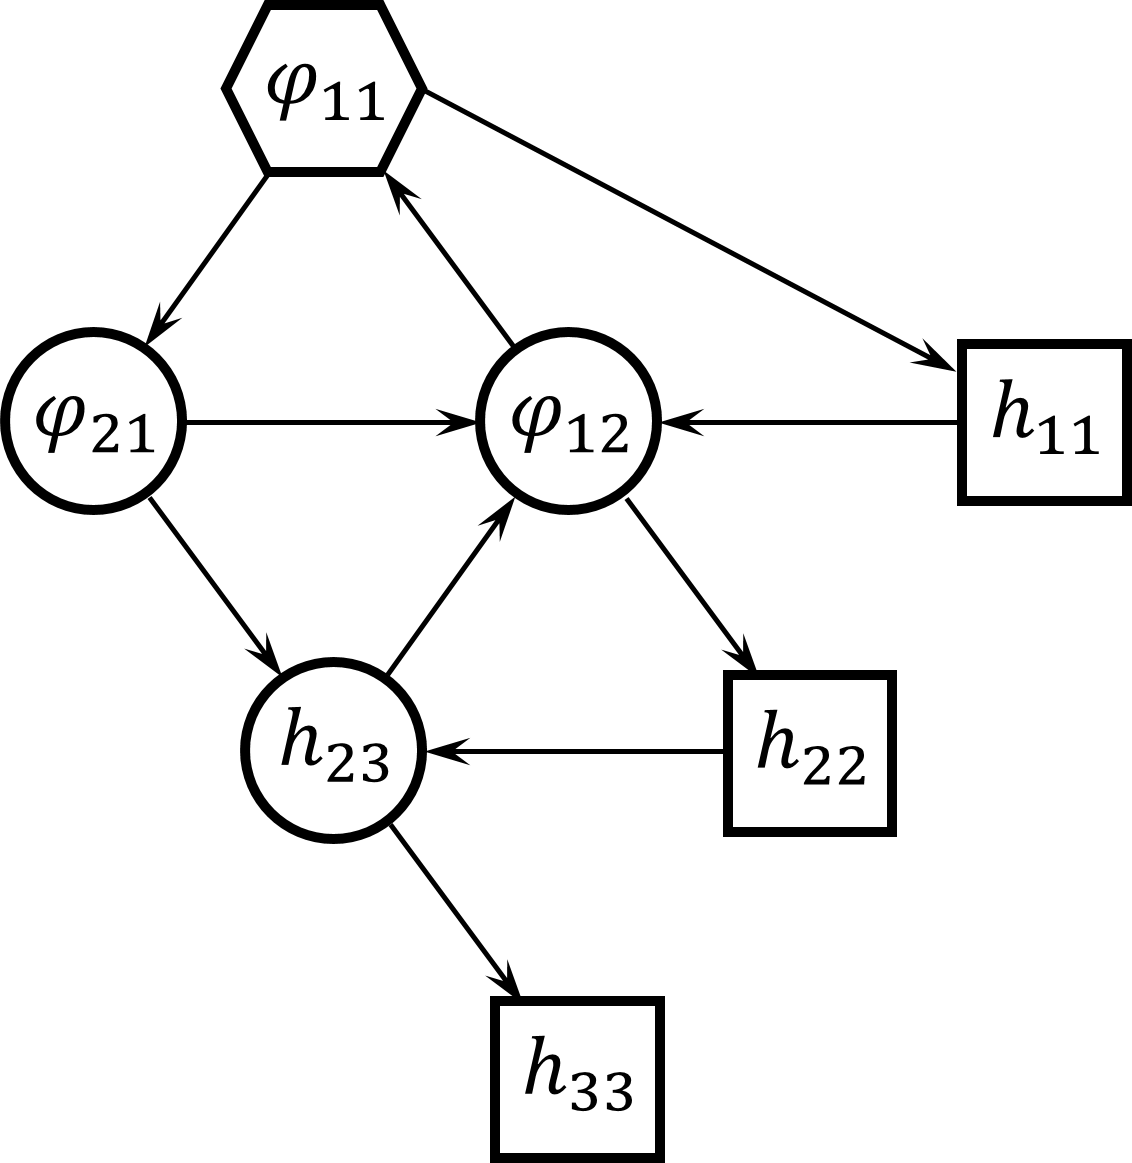
\includegraphics[scale=0.65]{h_convention/h_n=3_std.png}
\end{center}
\caption{The initial quiver for $\gc_h^{\dagger}(\bg_{\std},\GL_3)$. }
\label{f:h_n=3_std}
\end{figure}

\paragraph{The initial variables.} The variables in the initial extended cluster are given as follows:
\begin{equation}
    c_1(U) = \tr(U), \ \ c_2(U) = \frac{1}{2!} (\tr(U)^2 - \tr(U^2));
\end{equation}
\begin{equation}
    \varphi_{21}(U) = u_{13}, \ \ \varphi_{12}(U) = \det U^{[2,3]}_{[1,2]}\end{equation}\begin{equation}\varphi_{11}(U) = -\det \begin{bmatrix} u_{13} &(U^2)_{13}\\ u_{23} & (U^2)_{23}\end{bmatrix} =  u_{23}\det U^{[2,3]}_{[1,2]} + u_{13}\det U^{\{1,3\}}_{[1,2]};
\end{equation}
\begin{equation}
    h_{23}(U) = -u_{23}u_{33}-u_{13}u_{32}, \ \ h_{22}(U) = u_{33}\det U^{[2,3]}_{[2,3]} + u_{32}\det U^{[2,3]}_{\{1,3\}};
\end{equation}
\begin{equation}
    h_{11}(U) = \det U, \ \ h_{33}(U) = u_{33}.
\end{equation}

\paragraph{Some $1$-step mutations.} 
\begin{equation}
    \varphi_{11}^\prime(U) = \det \begin{bmatrix} u_{12} & u_{13}\\ (U^2)_{12} & (U^2)_{13}\end{bmatrix} = u_{12} \det U_{[1,2]}^{[2,3]} + u_{13} \det U_{\{1,3\}}^{[2,3]}.
\end{equation}
\subsection{$\Gamma_1 = \{2\}$, $\Gamma_2 = \{1\}$}
The initial quiver is illustrated in Figure~\ref{f:h_n=3_2-1}. 
\begin{figure}[htb]
\begin{center}
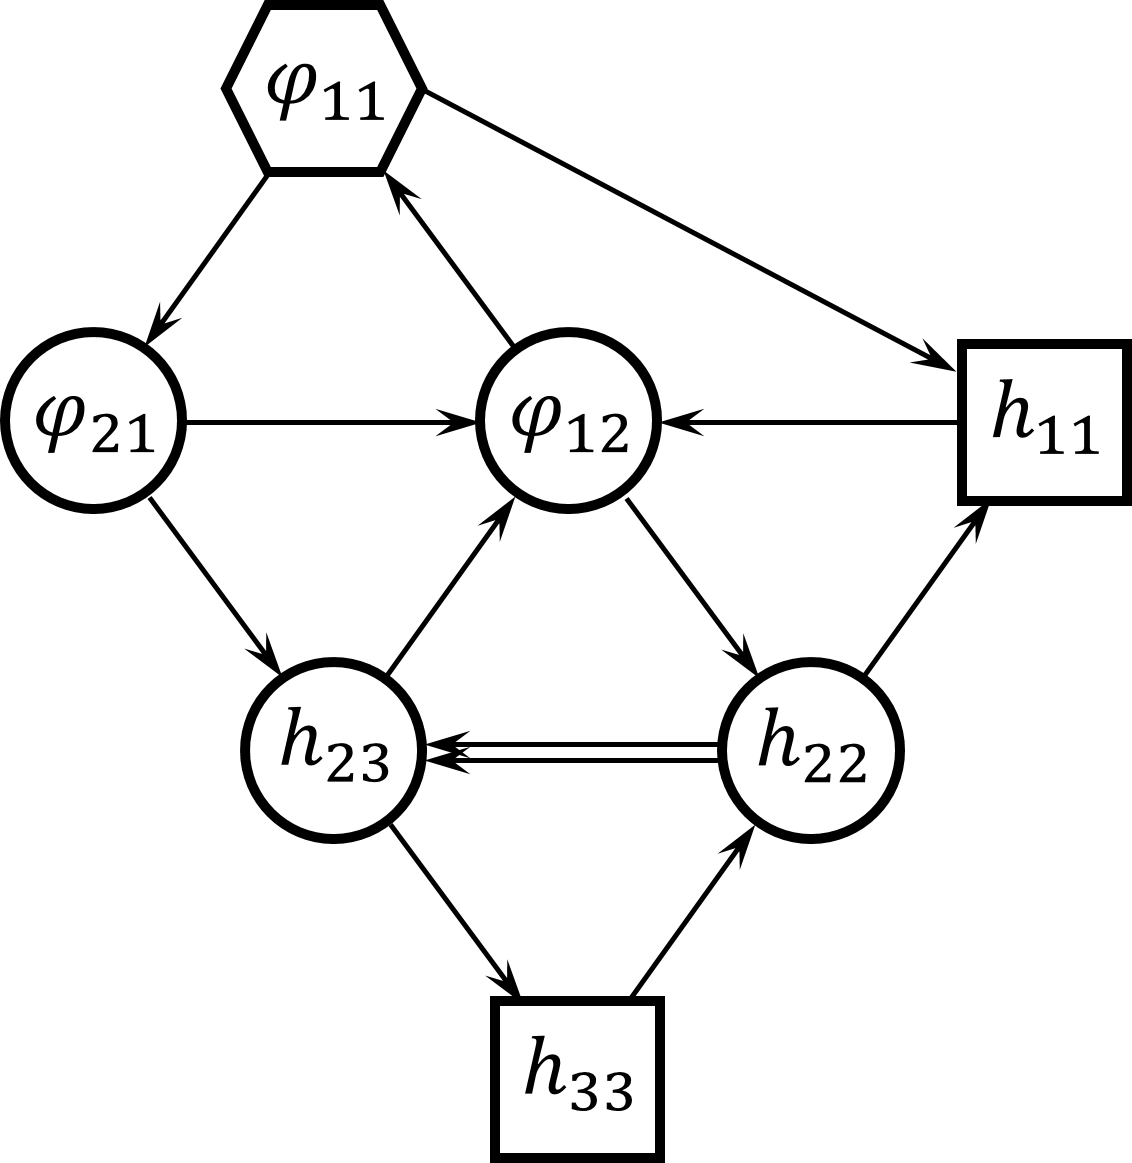
\includegraphics[scale=0.65]{h_convention/h_n=3_2-1.png}
\end{center}
\caption{The initial quiver for $\gc_h^{\dagger}(\bg,\GL_3)$ with $\Gamma_1 = \{2\}$, $\Gamma_2  = \{1\}$.}
\label{f:h_n=3_2-1}
\end{figure}

\paragraph{The initial variables.} All the variables in the initial extended cluster are as in $\gc_{h}^{\dagger}(\bg_{\std},\GL_3)$ except the variable $h_{33}$, which is given by
\begin{equation}
    h_{33}(U) = u_{33} \det U^{[2,3]}_{[2,3]} + u_{23} \det U_{[2,3]}^{\{1,3\}}.
\end{equation}

\paragraph{Birational quasi-isomorphisms.} The birational quasi-isomorphism \[\mathcal{Q}: (\GL_3,\gc_h^{\dagger}(\bg_{\std})) \dashrightarrow (\GL_3,\gc_h^{\dagger}(\bg))\]is given by
\begin{equation}
\mathcal{Q}(U)= (I-\alpha(U)e_{32})U(I+\alpha(U)e_{32}), \ \ \alpha(U):= \frac{\det U^{\{1,3\}}_{[2,3]}}{\det U^{[2,3]}_{[2,3]}}.
\end{equation}
\subsection{$\Gamma_1 = \{1\}$, $\Gamma_2 = \{2\}$}
The initial quiver is illustrated in Figure~\ref{f:h_n=3_1-2}. 
\begin{figure}[htb]
\begin{center}
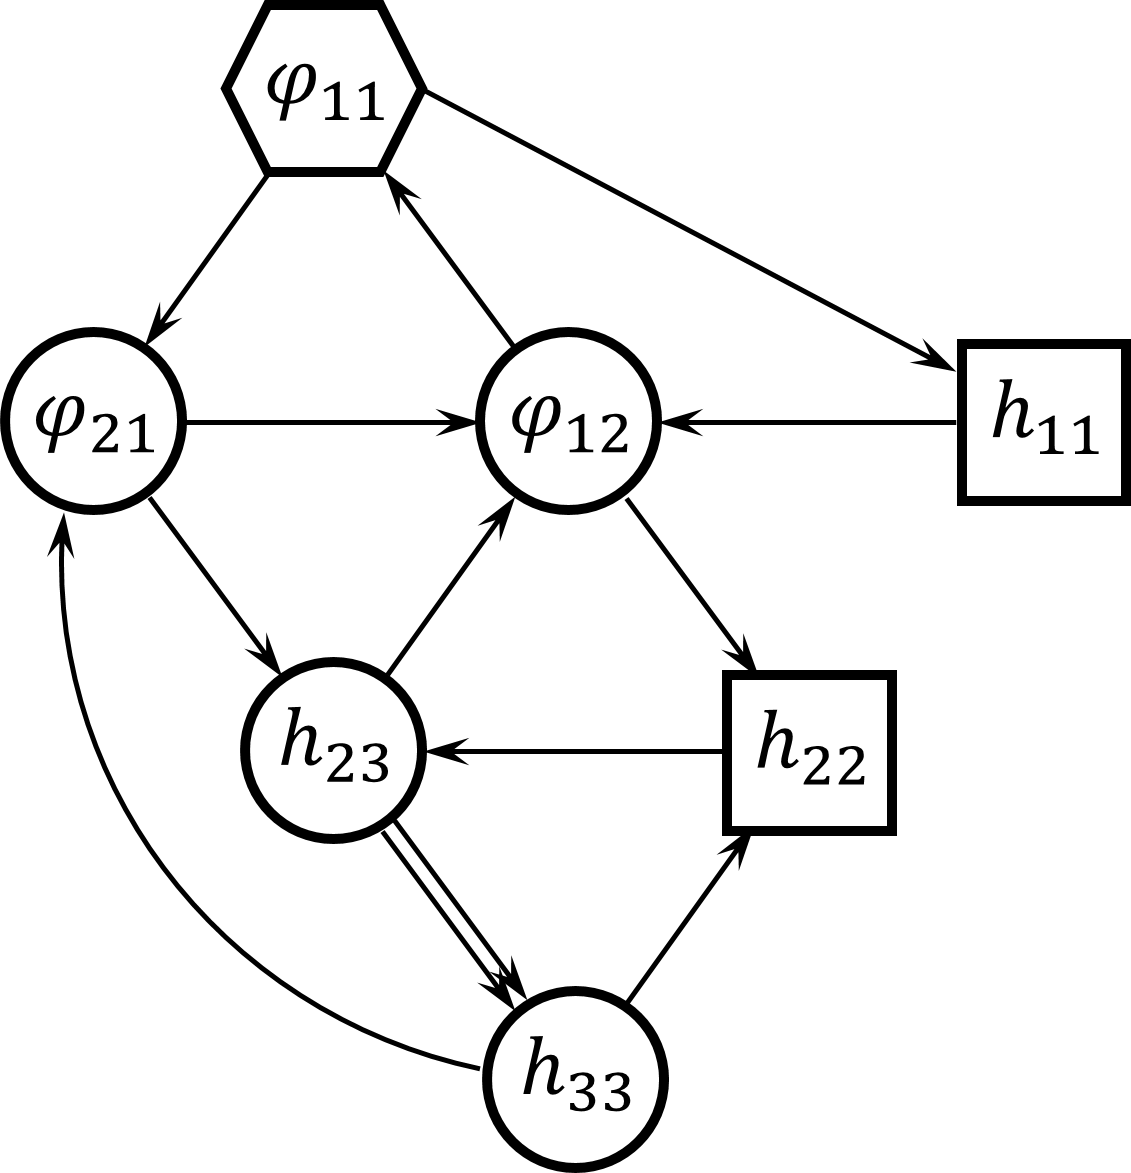
\includegraphics[scale=0.65]{h_convention/h_n=3_1-2.png}
\end{center}
\caption{The initial quiver for $\gc_h^{\dagger}(\bg,\GL_3)$ with $\Gamma_1 = \{1\}$, $\Gamma_2  = \{2\}$.}
\label{f:h_n=3_1-2}
\end{figure}

\paragraph{The initial variables.} All the variables in the initial extended cluster are as in $\gc_h^{\dagger}(\bg_{\std},\GL_3)$ except the variables $h_{23}$ and $h_{22}$; these are given by
\begin{equation}
    h_{23}(U) = -u_{23}u_{33}-u_{13}u_{32}, \ \ h_{22}(U) = u_{33} \det U^{[2,3]}_{[2,3]} + u_{32} \det U^{\{1,3\}}_{[2,3]}.
\end{equation}

\paragraph{Birational quasi-isomorphisms.} The birational quasi-isomorphism \[\mathcal{Q}:(\GL_3,\gc_h^{\dagger}(\bg_{\std}))\dashrightarrow (\GL_3,\gc_h^{\dagger}(\bg))\] is given by
\begin{equation}
    \mathcal{Q}(U) = (I-\alpha(U)e_{21})U(I+\alpha(U)e_{21}), \ \ \alpha(U):=\frac{u_{32}}{u_{33}}.
\end{equation}
\newpage
\section{Examples in $n=4$ in the $h$-convention}
\subsection{The standard BD triple}
The initial quiver for $\gc_h^{\dagger}(\bg_{\std},\GL_4)$ is illustrated in Figure~\ref{f:h_n=4_std}.

\begin{figure}[htb]
\begin{center}
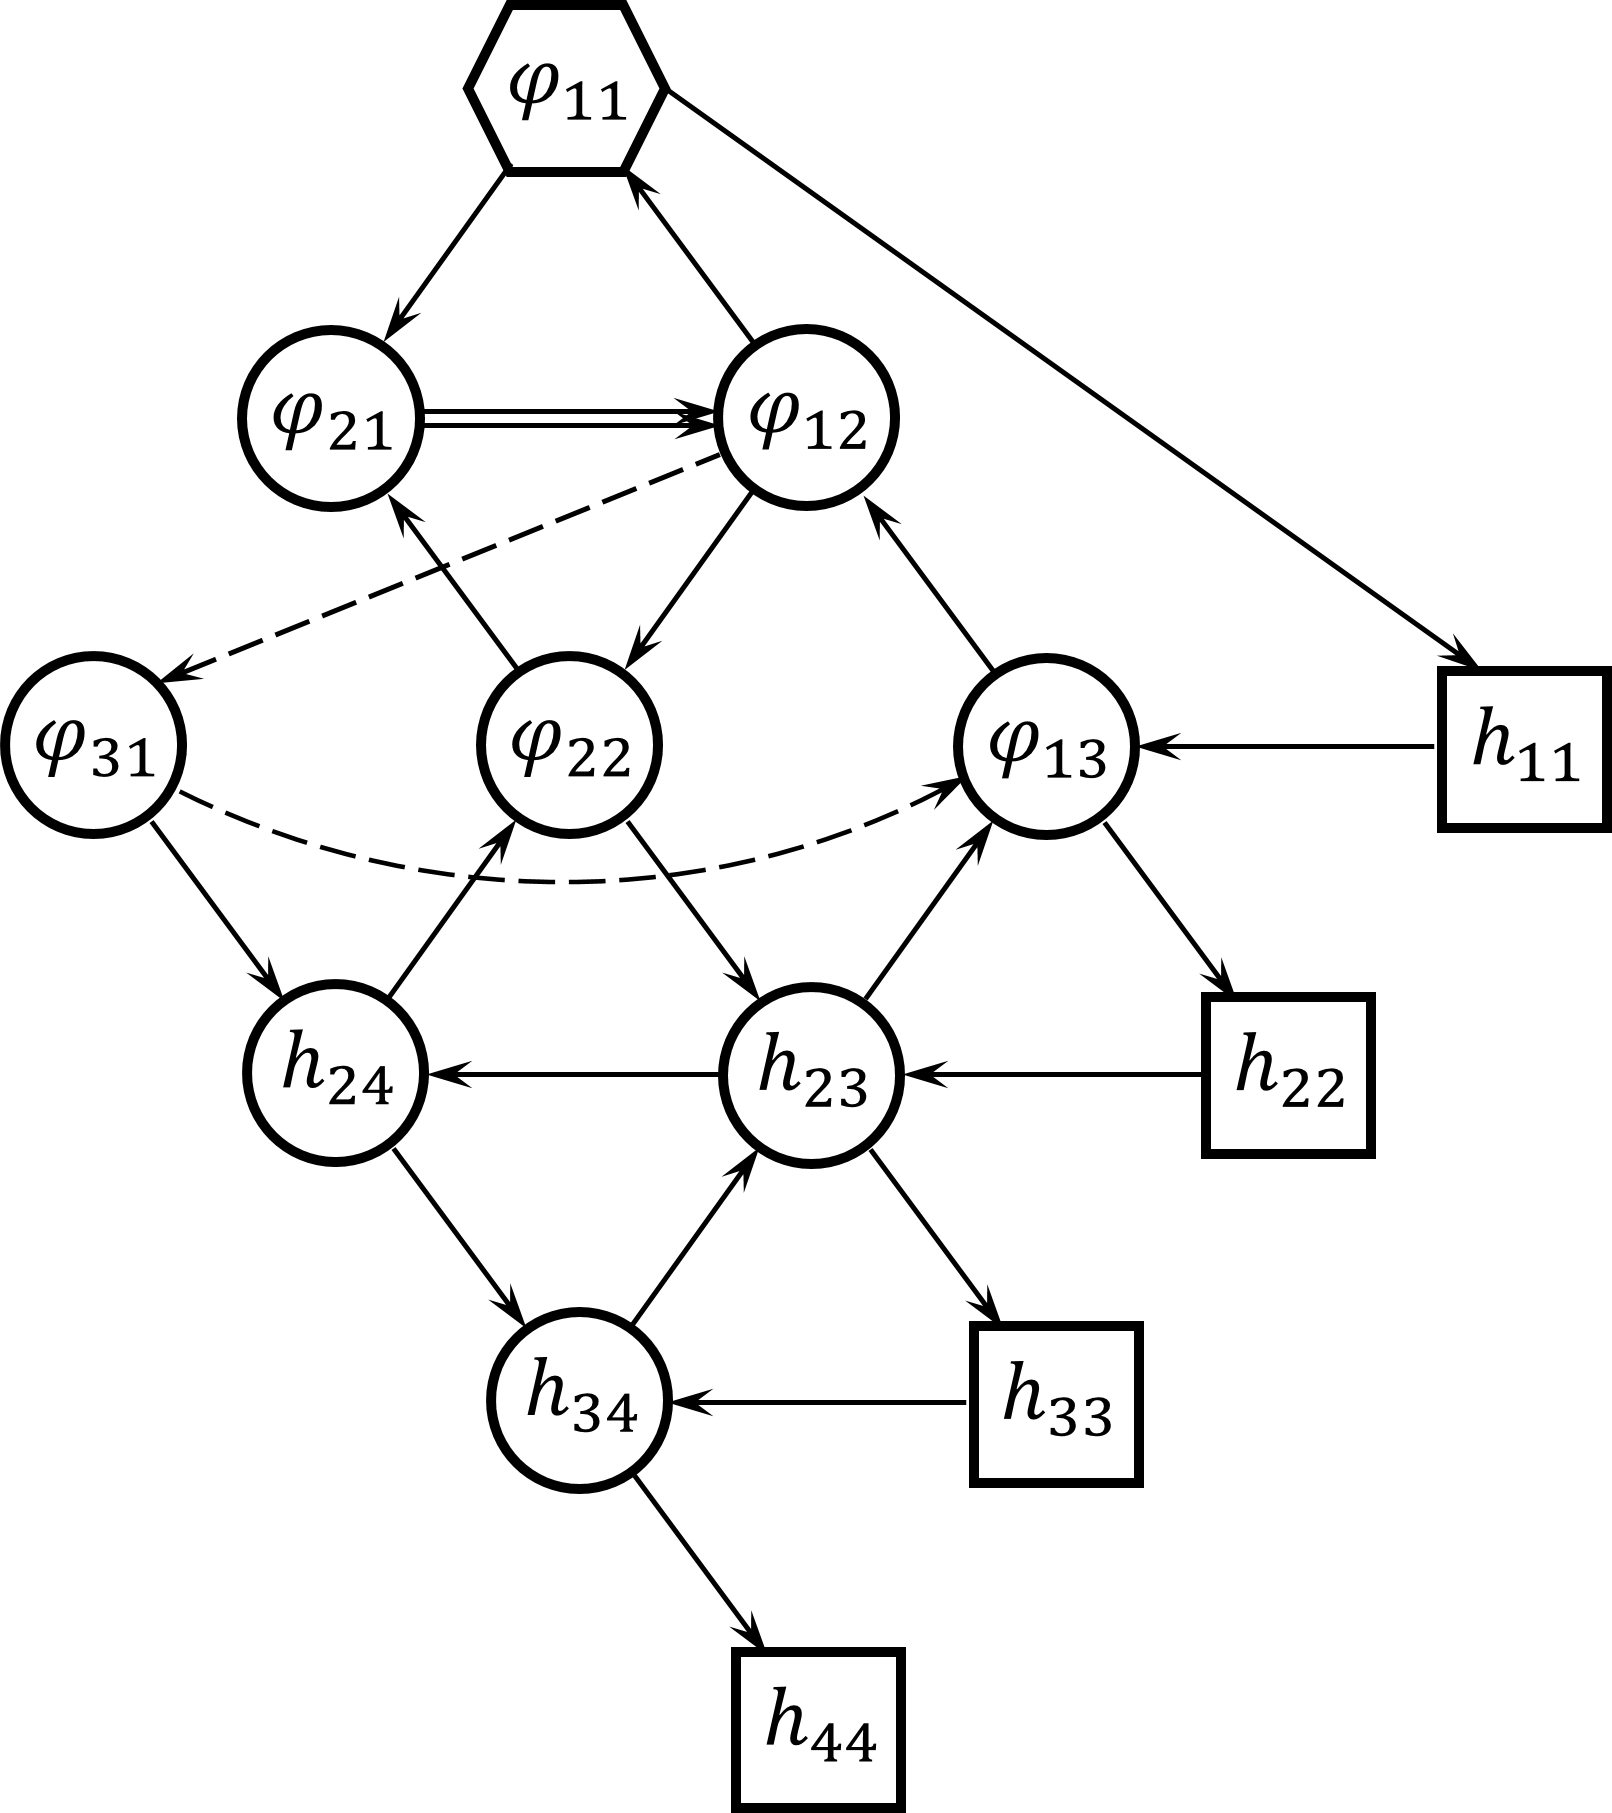
\includegraphics[scale=0.65]{h_convention/h_n=4_std.png}
\end{center}
\caption{The initial quiver for $\gc^{\dagger}_h(\bg_{\std},\GL_4)$.}
\label{f:h_n=4_std}
\end{figure}

\paragraph{The initial variables.} The $\varphi$-variables are given by
\begin{align}
    &\varphi_{11}(U) = -\det \begin{bmatrix}
        u_{14} & (U^2)_{14} & (U^3)_{14}\\
        u_{24} & (U^2)_{24} & (U^3)_{24}\\
        u_{34} & (U^2)_{34} & (U^3)_{34}
    \end{bmatrix};\\ &\varphi_{12}(U) =  \det \begin{bmatrix}
        u_{13} & u_{14} & (U^2)_{14}\\
        u_{23} & u_{24} & (U^2)_{24}\\
        u_{33} & u_{34} & (U^2)_{34}
    \end{bmatrix}, \ \ \varphi_{21}(U) = \det \begin{bmatrix}
        u_{14} & (U^2)_{14}\\ u_{24} & (U^2)_{24}
    \end{bmatrix};  \\
    &\varphi_{31}(U) = -u_{14}, \ \ \varphi_{22}(U) = \det U_{[1,2]}^{[3,4]}, \ \ \varphi_{13}(U) = - \det U_{[1,3]}^{[2,4]}.
\end{align}

The $h$-variables are given by
\begin{align}
    &h_{24}(U) = u_{24}, \ \ h_{23}(U) = \det U_{[2,3]}^{[3,4]}, \ \ h_{22}(U) = \det U_{[2,4]}^{[2,4]};\\
    &h_{34}(U) = -u_{34}, \ \ h_{33}(U) = \det U_{[3,4]}^{[3,4]}, \ \ h_{44}(U) = u_{44}.
\end{align}

The $c$-variables are given by
\begin{align}
    &c_1(U) = -\tr U, \ \ c_2(U) = \frac{1}{2!}\left(\tr(U)^2 - \tr(U^2)\right),\\ &c_3(U) = -\frac{1}{3!}\left( \tr(U)^3 - 3\tr(U)\tr(U^2)+2\tr(U^3)\right).
\end{align}

\paragraph{List of $1$-step mutations.} Here's what one obtains after a $1$-step mutation of the initial cluster in each direction:
%-U(1,4)*det(U([2,3],[1,4]))-U(3,4)*det(U([2,3],[3,4]))-U(2,4)*det(U(2:3,[2,4])) )
\begin{align}
&\varphi_{12}^\prime(U) = \det U_{[1,2]}^{[3,4]} \det \begin{bmatrix}
    u_{14} & (U^2)_{14}\\ u_{34} & (U^2)_{34} 
\end{bmatrix} + \begin{bmatrix}
    u_{14} & (U^2)_{14}\\ u_{24} & (U^2)_{24} 
\end{bmatrix} \det U_{[1,2]}^{\{2,4\}};\\
&\varphi_{21}^\prime(U) = -\det \begin{bmatrix}
    u_{14} & (U^2)_{13} & (U^2)_{14}\\
    u_{24} & (U^2)_{23} & (U^2)_{24}\\
    u_{34} & (U^2)_{33} & (U^2)_{34}
\end{bmatrix};\\
    &\varphi_{31}^\prime(U) = -\det U_{[1,3]}^{\{1\}\cup[3,4]}, \ \ 
\varphi_{31}^\prime(U) = -u_{24}\det U_{[2,4]}^{[2,4]} - u_{14} \det U_{[2,4]}^{\{1\}\cup[3,4]};\\&\varphi_{22}^\prime(U) = -u_{14}\det U_{[2,3]}^{\{1,4\}} - u_{24} \det U_{[2,3]}^{\{2,4\}} - u_{34} \det U_{[2,3]}^{[3,4]}.
\end{align}
\begin{align}
    &h_{24}^\prime(U) = -\det U_{\{1,3\}}^{[3,4]},\ \ \ h_{34}^\prime(U) = -\det U_{\{2,4\}}^{[3,4]};\\
    &h_{23}^\prime(U) = u_{14}\det U_{[2,4]}^{[2,4]} - u_{24} \det U_{\{1\}\cup[3,4]}^{[2,4]}.
\end{align}
 \subsection{Cremmer-Gervais $i \mapsto i+1$}
The initial quiver for $\gc_h^{\dagger}(\bg,\GL_4)$ is illustrated in Figure~\ref{f:n=4_CG_i-i+1}.

\begin{figure}[htb]
\begin{center}
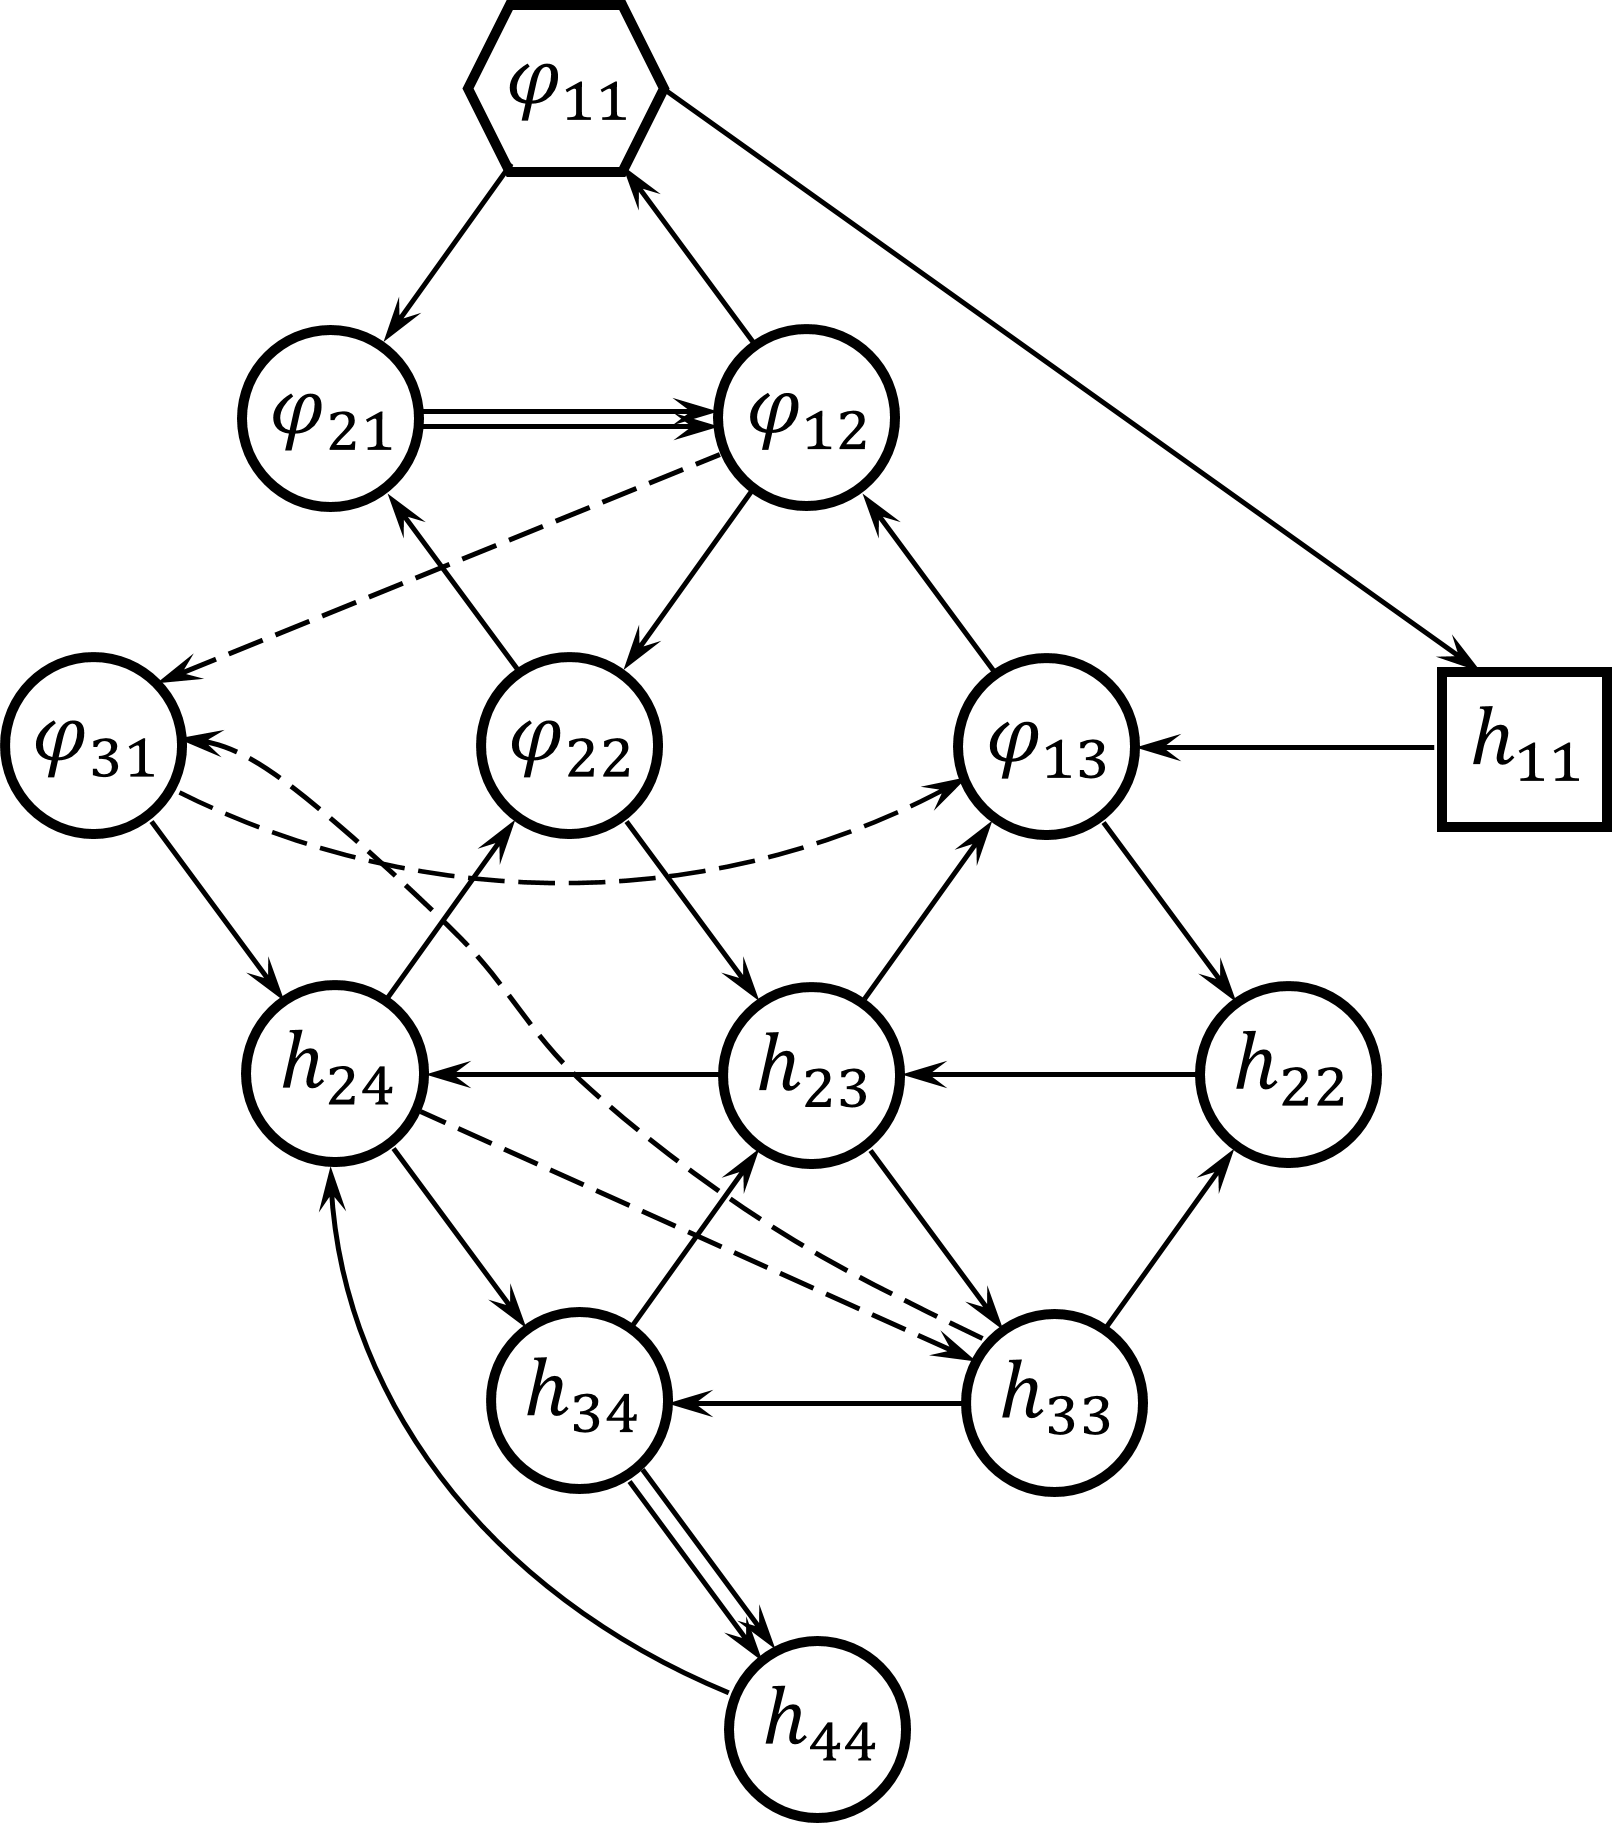
\includegraphics[scale=0.65]{h_convention/h_n=4_CG_i-i+1.png}
\end{center}
\caption{The initial quiver for $\gc^{\dagger}_g(\bg,\GL_4)$ for $\Gamma_1 = \{1,2\}$, $\Gamma_2 = \{2,3\}$, $\gamma:i \mapsto i+1$.}
\label{f:n=4_CG_i-i+1}
\end{figure}
 
 \paragraph{The initial variables.} In the initial extended cluster, all cluster and frozen variables are given as in $\gc_h^{\dagger}(\bg_{\std},\GL_4)$ except for the variables $h_{22}$, $h_{23}$, $h_{24}$, $h_{33}$, $h_{34}$. Let us set
\begin{align}
    &\ell_1(U) := \det U^{[3,4]}_{[3,4]}u_{44} +\det U_{\{2,4\}}^{[3,4]} u_{43}+ \det U^{[3,4]}_{\{1,4\}} u_{42};\\
    &\ell_2(U) := \det U_{[3,4]}^{\{2,4\}}u_{44} +\det U_{\{2,4\}}^{\{2,4\}} u_{43}+ \det U^{\{2,4\}}_{\{1,4\}} u_{42};\\
    &\ell_3(U) := \det U_{[3,4]}^{[2,3]}u_{44} +\det U_{\{2,4\}}^{[2,3]} u_{43}+ \det U^{[2,3]}_{\{1,4\}} u_{42}.
\end{align}
Then the $h$-variables are given by:
\begin{align}
    &h_{24}(U) = u_{24}\cdot \ell_1(U) + u_{14}\ell_2(U), \ \ h_{34}(U) = -u_{34}u_{44} - u_{24}u_{43} - u_{14}u_{42}, \ \ h_{44}(U) = u_{44}; \\
    &h_{23}(U) = \det U^{[3,4]}_{[2,3]}\ell_1(U) + \det U^{[3,4]}_{\{1,3\}}\ell_2(U) + \det U^{[3,4]}_{[1,2]}\ell_3(U), \ \ h_{33}(U) = \ell_1(U);\\
    &h_{22}(U) = \det U^{[2,4]}_{[2,4]}\ell_1(U) + \det U_{\{1\}\cup[3,4]}^{[2,4]}\ell_2(U) + \det U^{[2,4]}_{[1,2]\cup\{4\}}\ell_3(U).
\end{align}

 \paragraph{Birational quasi-isomorphisms.} TBD
 \subsection{Cremmer-Gervais $i \mapsto i-1$}
The initial quiver for $\gc_h^{\dagger}(\bg,\GL_4)$ is illustrated in Figure~\ref{f:n=4_CG_i-i-1}.

\begin{figure}[htb]
\begin{center}
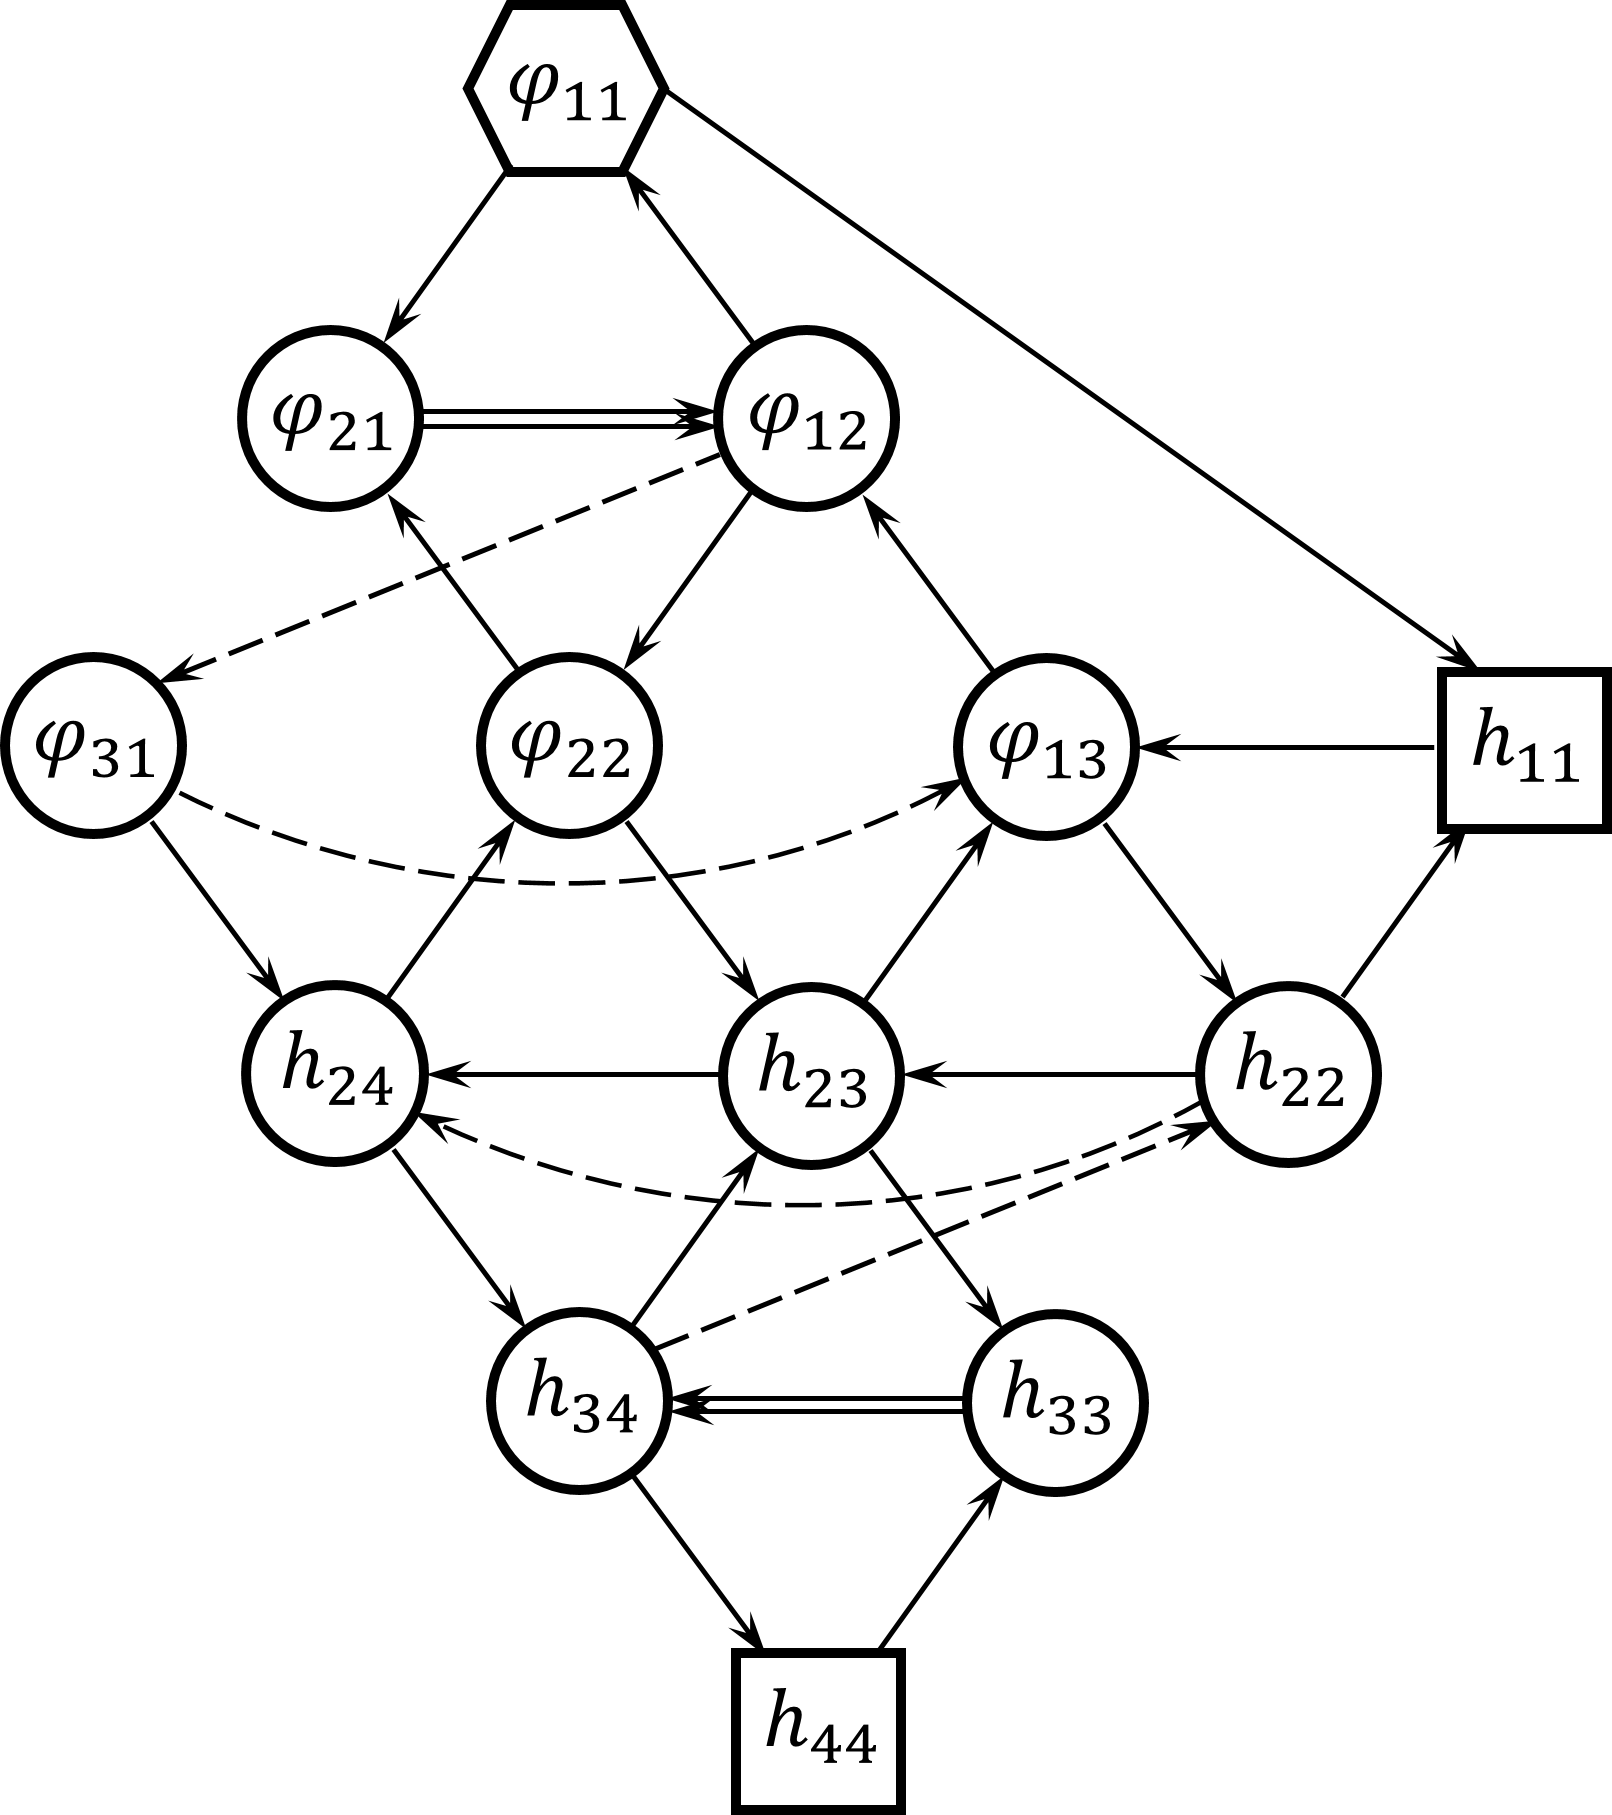
\includegraphics[scale=0.65]{h_convention/h_n=4_CG_i-i-1.png}
\end{center}
\caption{The initial quiver for $\gc^{\dagger}_h(\bg,\GL_4)$ for $\Gamma_1 = \{2,3\}$, $\Gamma_2 = \{1,2\}$, $\gamma:i \mapsto i-1$.}
\label{f:n=4_CG_i-i-1}
\end{figure}
 
 \paragraph{The initial variables.} In the initial extended cluster, all cluster and frozen variables are given as in $\gc_h^{\dagger}(\bg_{\std},\GL_4)$ except for the variables $h_{34}$, $h_{33}$, $h_{44}$. These are given by:
\begin{align}
    &h_{34}(U) = -u_{34}\det U^{[2,4]}_{[2,4]} - u_{24} \det U^{\{1\}\cup[3,4]}_{[2,4]};\\
    &h_{33}(U) = \det U^{[3,4]}_{[3,4]} \det U^{[2,4]}_{[2,4]} + \det U^{[3,4]}_{\{2,4\}} \det U^{\{1\}\cup[3,4]}_{[2,4]} + \det U^{[3,4]}_{[2,3]}\det U^{[1,2]\cup\{4\}}_{[2,4]};
\end{align}
\begin{equation}
    \begin{split}
     h_{44}(U) = &u_{44}\left(\det U^{[3,4]}_{[3,4]} \det U^{[2,4]}_{[2,4]} + \det U^{[3,4]}_{\{2,4\}} \det U^{\{1\}\cup[3,4]}_{[2,4]} + \det U^{[3,4]}_{[2,3]}\det U^{[1,2]\cup\{4\}}_{[2,4]}\right) + \\ + &u_{34}\left(\det U^{\{2,4\}}_{[3,4]} \det U^{[2,4]}_{[2,4]} + \det U^{\{2,4\}}_{\{2,4\}} \det U^{\{1\}\cup[3,4]}_{[2,4]} + \det U^{\{2,4\}}_{[2,3]}\det U^{[1,2]\cup\{4\}}_{[2,4]}\right) + \\ + &u_{24}\left(\det U^{\{1,4\}}_{[3,4]} \det U^{[2,4]}_{[2,4]} + \det U^{\{1,4\}}_{\{2,4\}} \det U^{\{1\}\cup[3,4]}_{[2,4]} + \det U^{\{1,4\}}_{[2,3]}\det U^{[1,2]\cup\{4\}}_{[2,4]}\right).
    \end{split}
\end{equation}

\paragraph{Birational quasi-isomorphisms.} TBD
\newpage
\section{Examples in $n=4$ in the $g$-convention}
\subsection{The standard BD triple}
The initial quiver for $\gc_g^{\dagger}(\bg_{\std},\GL_4)$ is illustrated in Figure~\ref{f:ex_n=4gstd}.

\begin{figure}[htb]
\begin{center}
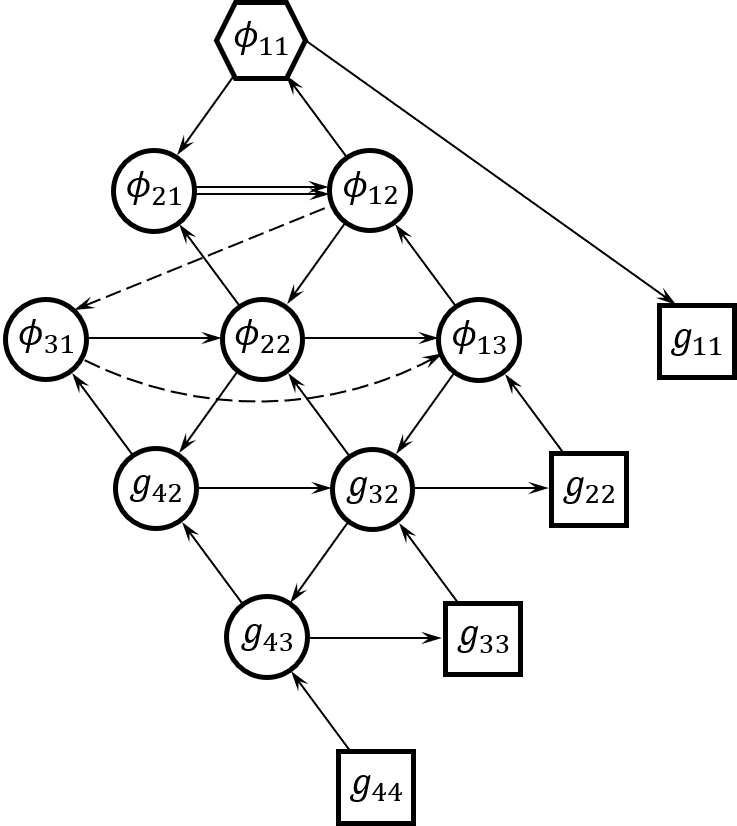
\includegraphics[scale=0.65]{g_convention/g_n=4_std.png}
\end{center}
\caption{The initial quiver for $\gc^{\dagger}_g(\bg_{\std},\GL_4)$.}
\label{f:ex_n=4gstd}
\end{figure}

\paragraph{The initial variables.} The $\phi$- and $c$-variables, as elements of $\mathcal{O}(\GL_4)$, are given by the following formulas:
\begin{align}
    \phi_{11}(U) = \det \begin{bmatrix} u_{21} & (U^2)_{21} & (U^3)_{21} \\ u_{31} & (U^2)_{31} & (U^3)_{31}\\ u_{41} & (U^2)_{41} & (U^3)_{41} \end{bmatrix}, \ \ \phi_{12}(U) = -\det\begin{bmatrix}u_{21} & u_{22} & (U^2)_{21}\\ u_{31} & u_{32} & (U^2)_{31}\\ u_{41} & u_{42} & (U^2)_{41} \end{bmatrix};\\
    \phi_{21}(U) = \det \begin{bmatrix}
        u_{31} & (U^2)_{31} \\ u_{41} & (U^2)_{41}
    \end{bmatrix}, \ \ \phi_{31}(U) = u_{41}, \ \ \phi_{22}(U) = \det U^{[1,2]}_{[3,4]}, \ \ \phi_{13}(U) = \det U^{[1,3]}_{[2,4]};
\end{align}
\begin{align}
    &c_1(U) = -\tr U, \ \ c_2(U) = \frac{1}{2!}\left(\tr(U)^2 - \tr(U^2)\right),\\ &c_3(U) = -\frac{1}{3!}\left( \tr(U)^3 - 3\tr(U)\tr(U^2)+2\tr(U^3)\right).
\end{align}
The $g$-variables are given by
\begin{equation}
    g_{11}(U):=\det U, \ \ g_{ij}(U) = \det U^{[j,n-i+j]}_{[i,n]}, \ \ 2 \leq j \leq i \leq n.
\end{equation}
\subsection{Cremmer-Gervais $i \mapsto i-1$}
The initial quiver for $\gc_g^{\dagger}(\bg,\GL_4)$ is illustrated in Figure~\ref{f:ex_n=4cg}.

\begin{figure}[htb]
\begin{center}
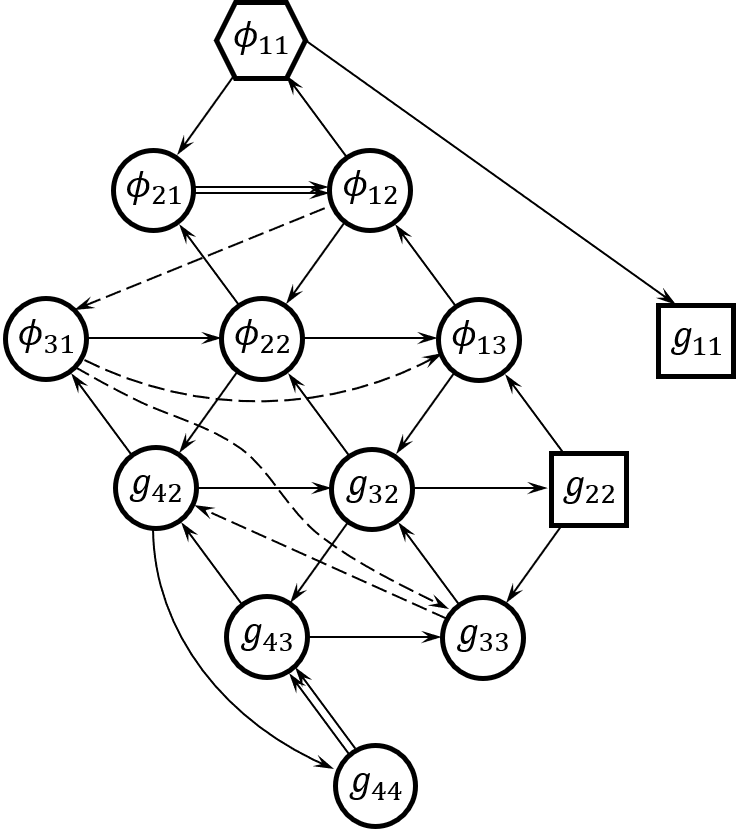
\includegraphics[scale=0.65]{g_convention/g_n=4_cg_i-i-1.png}
\end{center}
\caption{The initial quiver for $\gc^{\dagger}_g(\bg,\GL_4)$ for $\Gamma_1 = \{2,3\}$, $\Gamma_2 = \{1,2\}$, $\gamma:i \mapsto i-1$.}
\label{f:ex_n=4cg}
\end{figure}

\paragraph{The initial variables.} Let us set
\begin{align}
    &\ell_1(U) := \det U^{[3,4]}_{[3,4]}u_{44} +\det U^{\{2,4\}}_{[3,4]} u_{34}+ \det U_{[3,4]}^{\{1,4\}} u_{24};\\
    &\ell_2(U) := \det U^{[3,4]}_{\{2,4\}}u_{44} +\det U^{\{2,4\}}_{\{2,4\}} u_{34}+ \det U_{\{2,4\}}^{\{1,4\}} u_{24};\\
    &\ell_3(U) := \det U^{[3,4]}_{[2,3]}u_{44} +\det U^{\{2,4\}}_{[2,3]} u_{34}+ \det U_{[2,3]}^{\{1,4\}} u_{24}.
\end{align}
The $g$-variables are given by the following formulas:
\begin{align}
    &g_{42}(U) = u_{42}\cdot \ell_1(U) + u_{41}\ell_2(U), \ \ g_{43}(U) = u_{43}u_{44} + u_{42}u_{34} + u_{41}u_{24}, \ \ g_{44}(U) = u_{44}; \\
    &g_{32}(U) = \det U_{[3,4]}^{[2,3]}\ell_1(U) + \det U_{[3,4]}^{\{1,3\}}\ell_2(U) + \det U_{[3,4]}^{[1,2]}\ell_3(U), \ \ g_{33}(U) = \ell_1(U);\\
    &g_{22}(U) = \det U_{[2,4]}^{[2,4]}\ell_1(U) + \det U^{\{1\}\cup[3,4]}_{[2,4]}\ell_2(U) + \det U_{[2,4]}^{[1,2]\cup\{4\}}\ell_3(U).
\end{align}

\paragraph{Birational quasi-isomorphisms.} There is a birational quasi-isomorphism
\begin{equation}
    \mathcal{Q}^{\op}: (\GL_4,\gc_g^{\dagger}(\bg_{\std})) \dashrightarrow (\GL_4,\gc_g^{\dagger}(\bg)), \ \ \mathcal{Q}^{\op}(U):=\rho^{\op}(U)U (\rho^{\op}(U))^{-1}
\end{equation}
where the rational map $\rho^{\op}:\GL_n \dashrightarrow \GL_n$ is given by
\begin{equation}
    \rho^{\op}(U) = \left(I+\frac{u_{34}}{u_{44}}e_{12}\right)\cdot \left(I + \frac{\det U_{\{2,4\}}^{[3,4]}}{\det U^{[3,4]}_{[3,4]}}e_{12} + \frac{u_{24}}{u_{44}}e_{13} + \frac{u_{34}}{u_{44}}e_{23}\right).
\end{equation}
The marked variables for $\mathcal{Q}^{\op}$ are $g_{33}$ and $g_{44}$. Define the BD triples $\tilde{\bg}:=(\{2\},\{1\},2\mapsto 1)$ and $\hat{\bg}:=(\{3\},\{2\},3\mapsto 2)$. There is a pair of complementary birational quasi-isomorphisms 
\begin{equation}\mathcal{G}:(\GL_4,\gc_g^{\dagger}(\tilde{\bg})\dashrightarrow (\GL_4,\gc_g^{\dagger}(\bg)), \ \ \mathcal{G}^\prime:(\GL_4,\gc_g^{\dagger}(\hat{\bg})) \dashrightarrow (\GL_4,\gc_g^{\dagger}(\bg)).
\end{equation}
They are given by
\begin{align}
    \mathcal{G}^{\op}(U) &= G^{\op}(U)\cdot U \cdot G^{\op}(U)^{-1}, \ \ G^{\op}(U) := \left(I+\frac{u_{34}}{u_{44}}e_{12}\right)\cdot \left(I+\frac{u_{24}}{u_{44}}e_{13} + \frac{u_{34}}{u_{44}}e_{23}\right);
    \end{align}
    \begin{align}
   (\mathcal{G}^\op)^\prime(U) &= G^\prime(U)\cdot U \cdot G^{\prime}(U)^{-1}, \ \ G^{\prime}(U) := (I+\alpha_1(U) e_{12} + \alpha_2(U) e_{13}),\\
    \alpha_1(U) &= \frac{\det U^{[3,4]}_{\{2,4\}}u_{44} + \det U_{\{2,4\}}^{\{2,4\}}u_{34}}{\det U^{[3,4]}_{[3,4]}u_{44} + \det U_{[3,4]}^{\{2,4\}}u_{34}}, \ \ \alpha_2(U) = -\frac{\det U^{[3,4]}_{[2,3]}u_{44} + \det U_{[2,3]}^{\{2,4\}}u_{34}}{\det U^{[3,4]}_{[3,4]}u_{44} + \det U_{[3,4]}^{\{2,4\}}u_{34}}.
\end{align}
The marked variable for $\mathcal{G}$ is $g_{44}$, and the marked variable for $\mathcal{G}^\prime$ is $g_{33}$.

%The full description of $\gc_g^{\dagger}(\tilde{\bg})$ and $\gc_g^{\dagger}(\hat{\bg})$ (along with more examples) is available on the author's github repository (see the previous section).


%\newpage
%\clearpage
%\newpage
\begin{thebibliography}{99}
%\bibitem{bd} A. Belavin and V. Drinfeld, 'Solutions of the classical Yang-Baxter equation for simple Lie algbras', \emph{Funktsional. Anal. i Prilozhen} \textbf{16}(1982), 159--180. \doi{10.1007/BF01081585}

%\bibitem{bd2} A. Belavin and V. Drinfeld, \emph{{T}riangle {E}quations and {S}imple {L}ie {A}lgebras} (Hardwood Academic, 1998).

%\bibitem{upper_bounds} A. Berenstein, S. Fomin and A. Zelevinsky, 'Cluster algebras III: Upper bounds and double Bruhat cells', \emph{Duke Math. J.} \textbf{126}(1) (2005), 1--52. \doi{10.1215/S0012-7094-04-12611-9}

%\bibitem{bfz_param} A. Berenstein, S. Fomin and A. Zelevinsky, 'Parametrizations of canonical bases and totally positive matrices', \emph{Adv. Math.} \textbf{122}(1) (1996), 49--149. \doi{10.1006/aima.1996.0057}

% \bibitem{berenstein2005quantum} A. Berenstein and A. Zelevinsky, 'Quantum cluster algebras', \emph{Adv. Math.} \textbf{195}(2005), 405--455.\\ \doi{10.1016/j.aim.2004.08.003}

%\bibitem{dual_brahami}R. Brahami, 'Cluster $\Chi$-varieties for dual Poisson-Lie groups, I', \emph{Algebra i Analiz} \textbf{22}(2) (2010), 14--104.
%\doi{10.1090/S1061-0022-2011-01138-0}

%\bibitem{chari} V. Chari and A. Pressley, \emph{A {G}uide to {Q}uantum {G}roups} (Cambridge Univ. Press, 1995).

%  \bibitem{earlier} L. Chekhov and M. Shapiro, 'Teichm{\"u}ller spaces of Riemann surfaces with orbifold points of arbitrary order and cluster variables' \emph{Int. Math. Res. Not. IMRN} \textbf{10} (2014), 2746--2772.\\ \doi{10.1093/imrn/rnt016}

%\bibitem{bdr} P. Delorme, 'Classification des triples de Manin pour les algebres de Lie reductives complexes: Avec un appendice de Guillaume Macey', \emph{J. Algebra} \textbf{246}(1) (2001), 97--174.\\ \doi{10.1006/jabr.2001.8887}

%\bibitem{slfive} I. Eisner, 'Exotic cluster structures on $\SL_5$', \emph{J. Phys. A} \textbf{47}(2014) 474002.\\ {\doi{10.1088/1751-8113/47/47/474002}}

% \bibitem{etingof} P. Etingof and O. Schiffmann, \emph{Lectures on {Q}uantum {G}roups} (International Press, 1998).

%\bibitem{etingofdyn} P. Etingof, T. Schedler, O. Schiffmann, 'Explicit quantization of dynamical r-matrices for finite dimensional semisimple Lie algebras', \emph{J. Amer. Math. Soc.} \textbf{13}(3) (2000), 595--609. \\ \doi{10.1090/S0894-0347-00-00333-7}

%\bibitem{fockcoords} V. Fock and A. Goncharov, 'Moduli spaces of local systems and higher Teichm\"uller theory', \emph{Publ. Math. Inst. Hautes \'Etudes Sci.} \textbf{103}(2006), 1--211.

%  \bibitem{fock2006cluster}
% V. Fock and A. Goncharov, 'Cluster $\chi$-varieties, amalgamation, and Poisson-Lie groups', \emph{Progr. Math.} \textbf{253}(2006), 27--68. \doi{10.1007/978-0-8176-4532-8_2}

% \bibitem{tensordiags} S. Fomin and P. Pylyavskyy, 'Tensor diagrams and cluster algebras', \emph{Adv. Math.} \textbf{300}(10) (2016), 717--787. \\ \doi{10.1016/j.aim.2016.03.030}

% \bibitem{fraser} C. Fraser, 'Quasi-Homomorphisms of Cluster Algebras', \emph{Adv. in Appl. Math.} \textbf{81}(2016), 40--77. \\\doi{10.1016/j.aam.2016.06.005}

%\bibitem{fomin6} S. Fomin, L. Williams and A. Zelevinsky, 'Introduction to Cluster algebras. Chapter 6', Preprint, 2020. \href{https://arxiv.org/abs/2008.09189}{arXiv:2008.09189}.
%\href{https://arxiv.org/abs/2008.09189}{\nolinkurl{arXiv:2008.09189}}. %<--- makes it bold and not beautiful

%\bibitem{fathers} S. Fomin and A. Zelevinsky, 'Cluster algebras I: Foundations', \emph{J. Amer. Math. Soc.} \textbf{15}(2) (2002), 497--529. \doi{10.1090/S0894-0347-01-00385-X}

%\bibitem{gantmacher} F. Gantmacher, \emph{The theory of matrices, vol. 1} (Amer. Math. Soc., Providence, RI, 1998)
%\bibitem{chari} V. Chari and A. Pressley, \emph{A {G}uide to {Q}uantum {G}roups} (Cambridge Univ. Press, 1995).

%\bibitem{rho} M. Gekhtman, M. Shapiro and A. Vainshtein, 'A unified approach to exotic cluster structures on simple Lie groups', Preprint, 2023. \href{https://arxiv.org/abs/2308.16701}{arXiv:2308.16701}.

%\href{https://arxiv.org/abs/2308.16701}{\nolinkurl{arXiv:2308.16701}}.

 %\bibitem{dasbuch} M. Gekhtman, M. Shapiro and A. Vainshtein, '{C}luster algebras and {P}oisson geometry', \emph{Math. Surveys Monogr.} \textbf{167}(2010). \doi{10.1090/surv/167}

%\bibitem{roots} M. Gekhtman, M. Shapiro and A. Vainshtein, 'Cluster algebras and Poisson geometry', \emph{Mosc. Math. J.} \textbf{3}(3) (2003), 899-934. \doi{10.17323/1609-4514-2003-3-3-899-934}; \href{https://arxiv.org/abs/math/0208033}{arXiv:0208033}.

%\bibitem{conj} M. Gekhtman, M. Shapiro and A. Vainshtein, 'Cluster structures on simple complex Lie groups and Belavin-Drinfeld classification', \emph{Mosc. Math. J.} \textbf{12}(2) (2010), 293--312. 
%% %\doi{10.17323/1609-4514-2012-12-2-293-312} %the doi is broken

% \bibitem{exotic}  M. Gekhtman, M. Shapiro, and A Vainshtein, 'Exotic cluster structures on $\SL_n$: the {C}remmer-{G}ervais case', \emph{Mem. Amer. Math. Soc.} \textbf{246}(1165) (2017), 1--94. \doi{10.1090/memo/1165}

\bibitem{double} M. Gekhtman, M. Shapiro and A. Vainshtein, 'Drinfeld double of $\GL_n$ and generalized cluster structures', \emph{Proc. Lond. Math. Soc.} \textbf{116}(3) (2018), 429--484. \doi{10.1112/plms.12086}

%\bibitem{doublerel} M. Gekhtman, M. Shapiro and A. Vainshtein, 'Generalized cluster structures related to the Drinfeld double of $\GL_n$', \emph{J. Lond. Math. Soc.} \textbf{105}(3), (2022),
%  1601--1633.\\ \doi{10.1112/jlms.12542}

%\bibitem{periodic} M. Gekhtman, M. Shapiro and A. Vainshtein, 'Periodic staircase matrices and generalized cluster structures', \emph{Int. Math. Res. Not. IMRN} \textbf{2022}(6) (2022), 4181--4221.\\ \doi{10.1093/imrn/rnaa148}

%\bibitem{plethora} M. Gekhtman, M. Shapiro and A. Vainshtein, 'Plethora of cluster structures on $\GL_n$', Preprint, 2019. \href{https://arxiv.org/abs/1902.02902}{arXiv:1902.02902}.

%\bibitem{grass_poiss} M. Gekhtman, M. Shapiro and A. Vainshtein, 'Poisson geometry of directed networks in a disk', \emph{Selecta Math. (N.S.)} \textbf{15} (2009), 61--103. \doi{10.1007/s00029-009-0523-z}

%\bibitem{yakimov_locus} K. R. Goodearl, M. T. Yakimov, 'Cluster algebra structures on Poisson nilpotent algebras', Preprint, 2018. \doi{10.48550/arXiv.1801.01963}

%\bibitem{ivan_ip} I. Ip, 'Cluster realization of $U_q(\mathfrak{g})$ and factorizations of the universal $R$-matrix, \emph{Selecta Math.} \textbf{24}(5) (2018), 4461--4553. \doi{10.1007/s00029-018-0432-0}

%\bibitem{hodges} T. J. Hodges, 'On the Cremmer-Gervais quantizations of $\SL(n)$', \emph{Int. Math. Res. Not. IMRN} \textbf{10} (1995), 465--481. \doi{10.1155/S107379289500033X}

%\bibitem{open_rich} B. Leclerc, 'Cluster structures on strata of flag varieties', \emph{Adv. Math.} \textbf{300}(10) (2016), 190--228.\\ \doi{10.1016/j.aim.2016.03.018}

%\bibitem{yakimov_det} B. Nguyen, K. Trampel and M. Yakimov, 'Noncommutative discriminants via Poisson primes', \emph{Adv. Math.} \textbf{322}(2017), 269--307. \doi{10.1016/j.aim.2017.10.018}

%\bibitem{rs}  A. Reyman and M. Semenov-Tian-Shansky, \emph{{I}ntegrable systems.} (Institute of Computer Studies, Moscow, 2003).

%\bibitem{serre} J.-P. Serre, \emph{Complex semisimple Lie algebras.} (Springer Science \& Business Media, New York, 1987).

%  \bibitem{schneider} H. Schneider, 'The concepts of irreducibility and full indecomposability of a matrix in the works of Frobenius, K{\"o}nig and Markov', \emph{Linear Algebra Appl.} \textbf{18}(12) (1977), 139--162. \doi{10.1016/0024-3795(77)90070-2} 

\bibitem{multdouble} D. Voloshyn, 'Multiple generalized cluster structures on $D(\mathrm{GL}_n)$', \emph{Forum of Mathematics, Sigma} \textbf{11}(46) (2023), 1--78. \doi{10.1017/fms.2023.44}

%\bibitem{zametka} D. Voloshyn, 'Starfish lemma via birational quasi-isomorphisms', Preprint, 2023. \\ \href{https://arxiv.org/abs/2311.00404}{arXiv:2311.00404}.

 \bibitem{multdual} D. Voloshyn and M. Gekhtman, 'Generalized cluster structures on $\SL_n^{\dagger}$', Preprint, 2023. \href{https://arxiv.org/abs/2312.04859}{arXiv:2312.04859}  

%\bibitem{sasha_group} G. Schrader and A. Shapiro, 'A cluster realization of $U_q(\sll_n)$ from quantum character varieties', \emph{Invent. Math} \textbf{216}(2019), 799--846. \doi{10.1007/s00222-019-00857-6}

%\bibitem{sasha_gauge} G. Schrader and A. Shapiro, '$K$-theoretic Coulomb branches of quiver gauge theories and cluster varieties', Preprint, 2019. \href{https://arxiv.org/abs/1910.03186}{arXiv:1910.03186}.

%\bibitem{scott} J. Scott, 'Grassmannians and cluster algebras', \emph{Proc. Lond. Math. Soc.} \textbf{92} (2006), 345--380. \\ \doi{10.1112/S0024611505015571}

%\bibitem{bott_shen} L. Shen and D. Weng, 'Cluster structures on double Bott-Samelson cells', \emph{Forum of Mathematics, Sigma} \textbf{9}(66) (2021), 1-89. \doi{10.1017/fms.2021.59}

%\bibitem{dual_shen} L. Shen, 'Duals of semisimple Poisson-Lie groups and cluster theory of moduli spaces of $G$-local systems', \emph{Int. Math. Res. Not. IMRN} \textbf{2022}(18), 14295--14318. \doi{10.1093/imrn/rnab094}

%1910.03186

\end{thebibliography}

\end{document}